\section{Results}\label{sec:exps}

\subsection{Models based on various features}

Описание экспериментов по построению моделей. Основная цель эксперимента - улучшение качества моделей за счет использования более глубоких данных. Базовая модель - SDSS. + описать сравнение моделей на, обученных на рентгеновской выборке vs обученных на оптической.

\subsection{Models based on various trains}

\subsection{Photometric errors}

Здесь про разыгрывание ошибок. Сначала описание 22ой модели, что у неё не скоррелированы признаки, поэтому можно спокойно разыгрывать ошибки (м.б. посчитать корелляцию Пирсона для всех признаков?), потом сравнение до-после по точности.

\begin{table}[ht]
    \centering
    \begin{tabular}{lcc}
    \hline
        Модель & $NMAD$ & $n_{>0.15}$ \\
    \hline
        Without perturbations & 0.037 & 0.110 \\
        8 perturbations (288 trees) & 0.033 & 0.101 \\
        16 perturbations (272 trees) & 0.034 & 0.109 \\
        32 perturbations (264 trees) & 0.035 & 0.110 \\
        32 perturbations (528 trees) & 0.035 & 0.112 \\
    \hline
    \end{tabular}
    \caption{Models with photometric errors accounting comparison on SDSS DR16 quasars with $z > 3$}
    \label{tab:perturbed}
\end{table}

\begin{figure*}
    \centering
    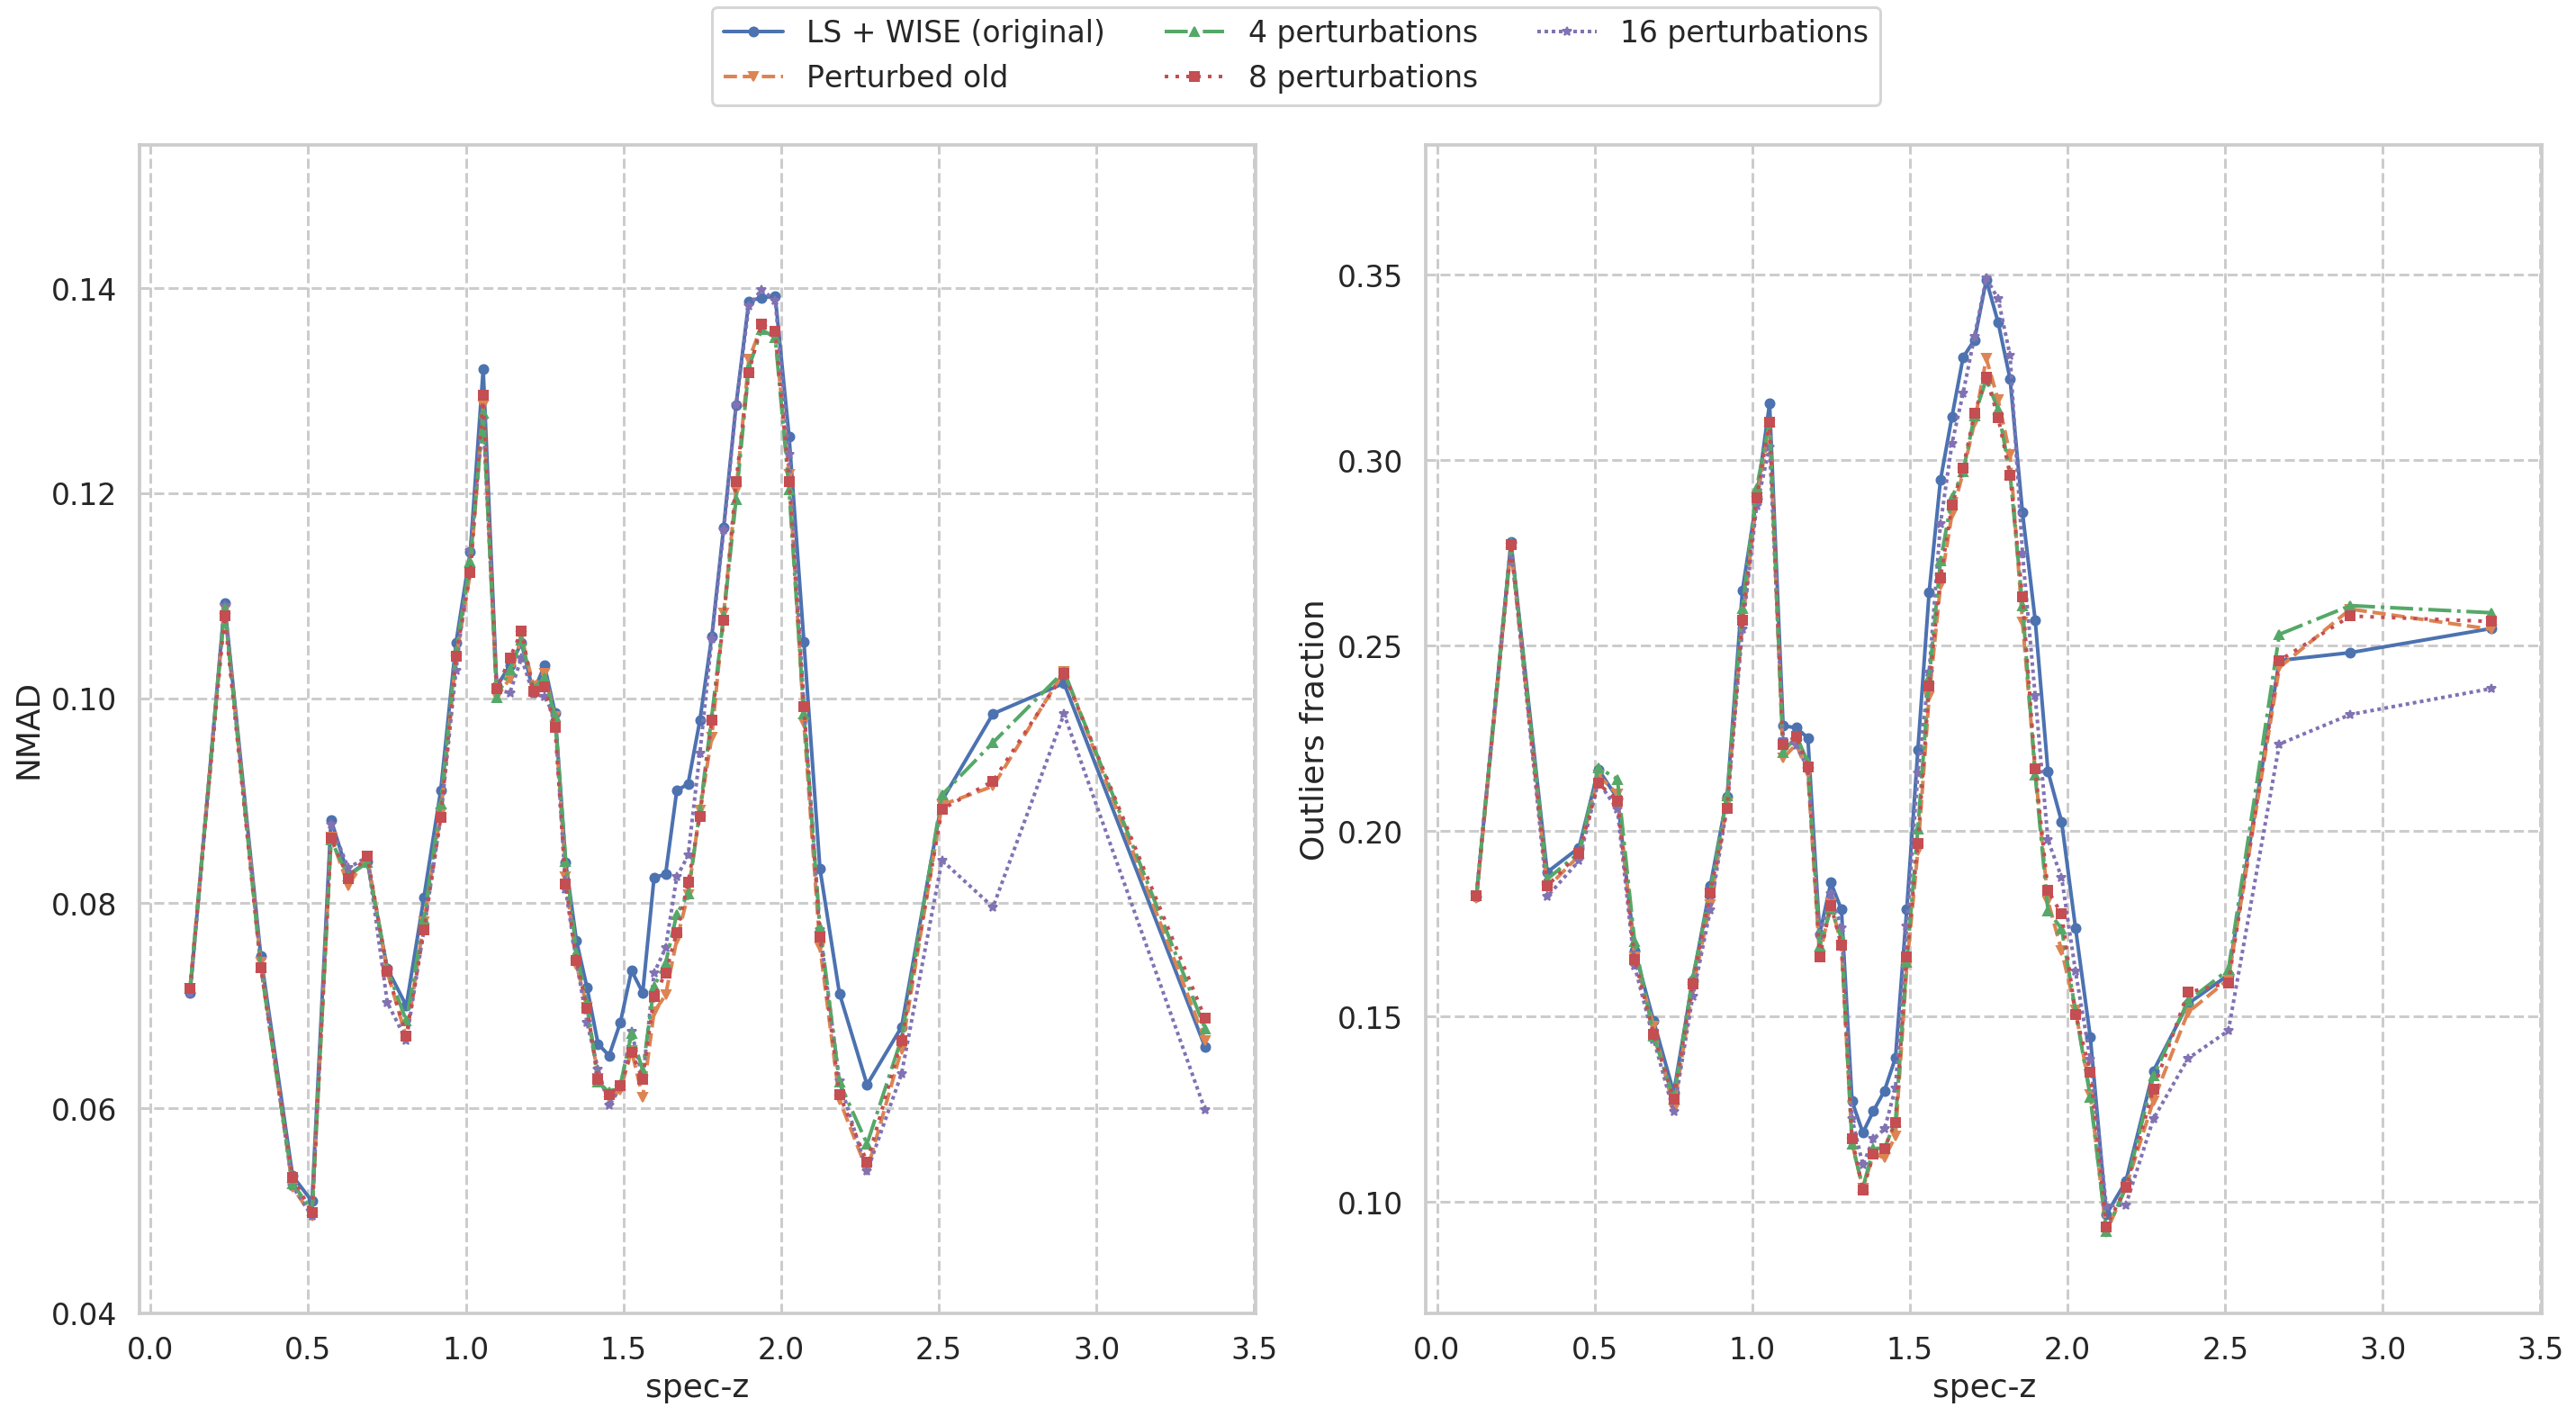
\includegraphics[width=\linewidth]{images/perturbations-22-zspec.png}
    \caption{DESI LIS + WISE model with different number of perturbations comparison on DR16 quasars by spec-z bins.}
    \label{fig:perturbations_22_zspec}
\end{figure*}

\begin{figure*}
    \centering
    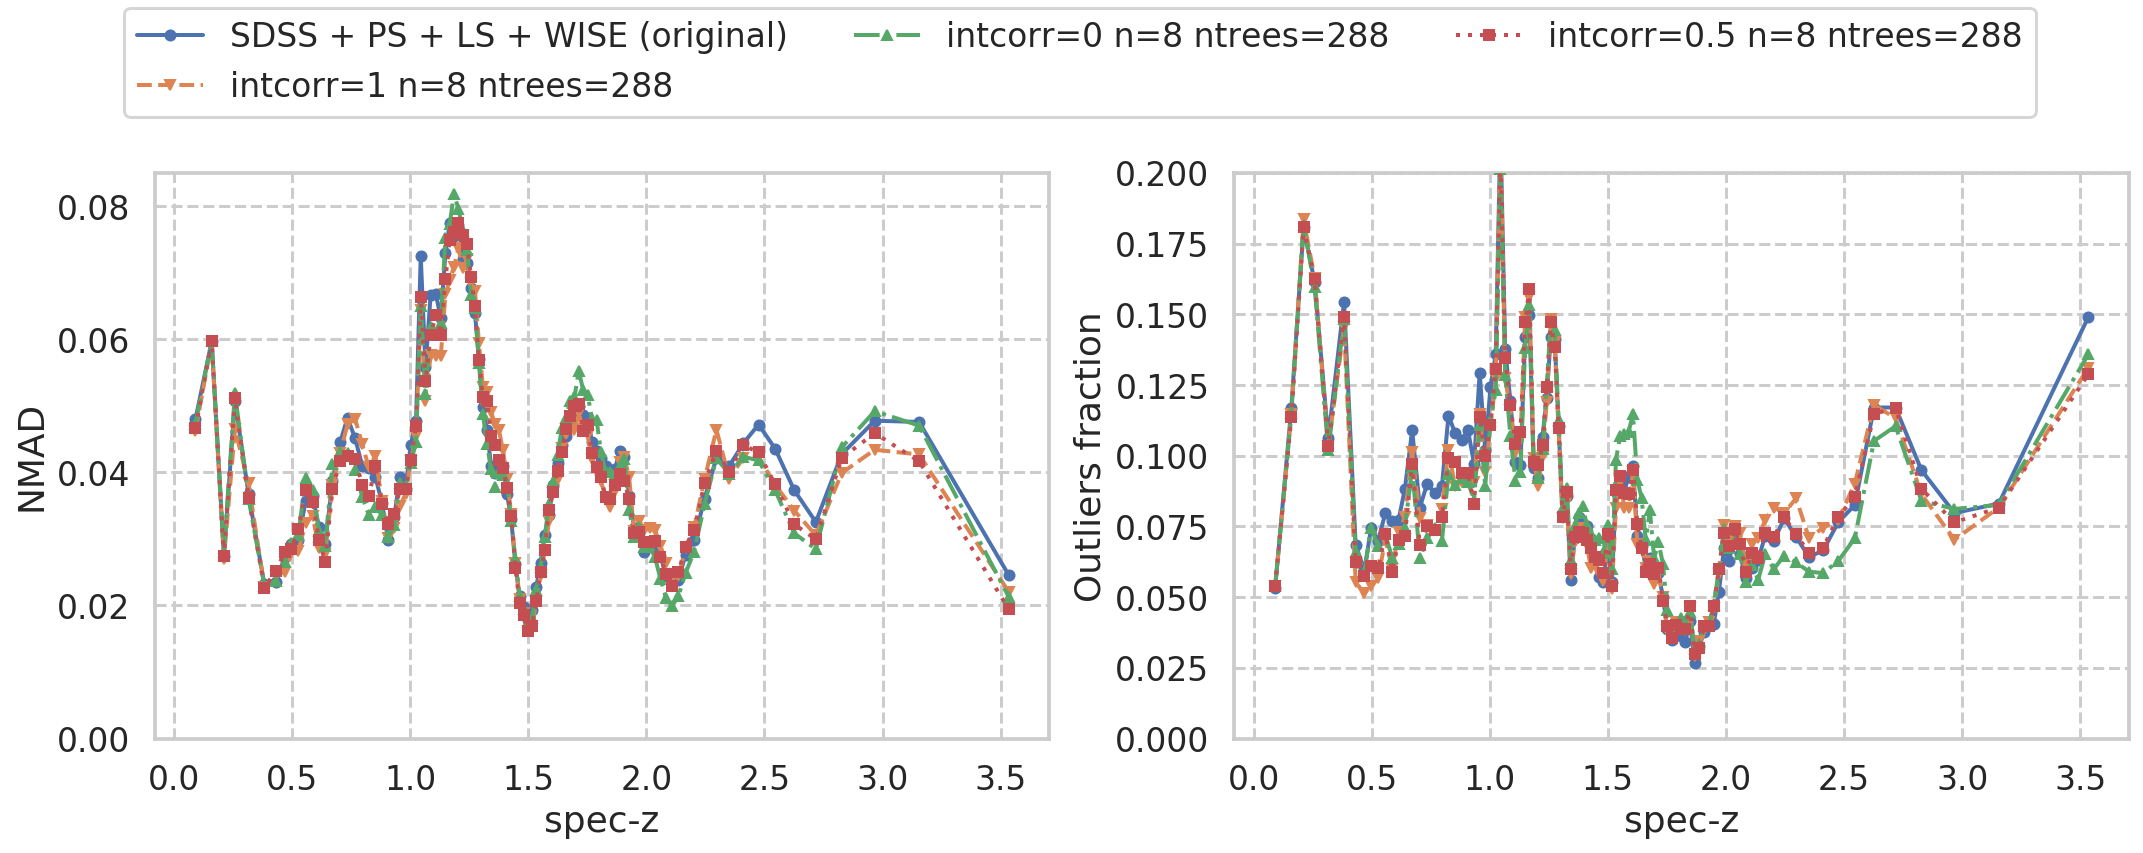
\includegraphics[width=\linewidth]{images/perturbations-intcorr-35-zspec.png}
    \caption{SDSS + PanSTARRS + DESI LIS + WISE model with different correlation inside filters comparison on DR16 quasars by spec-z bins.}
    \label{fig:perturbations_intcorr_35_zspec}
\end{figure*}

\begin{figure*}
    \centering
    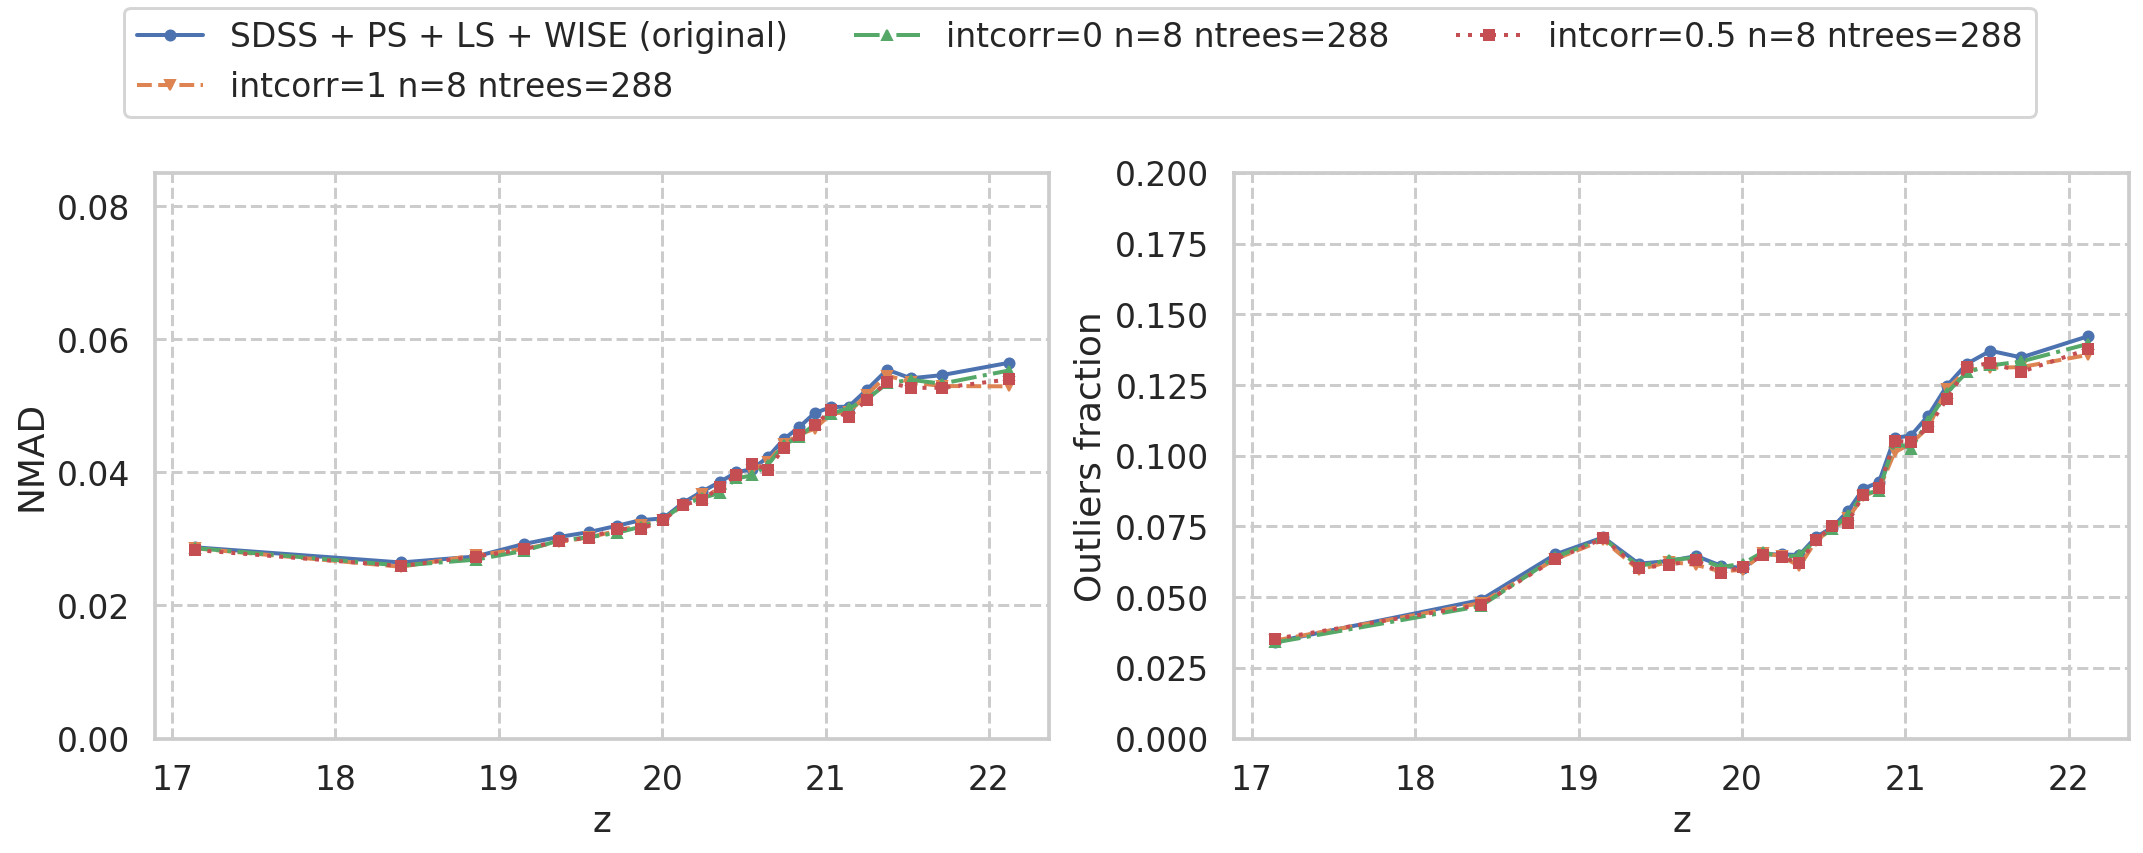
\includegraphics[width=\linewidth]{images/perturbations-intcorr-35-z.png}
    \caption{SDSS + PanSTARRS + DESI LIS + WISE model with different correlation inside filters comparison on DR16 quasars by z mag bins.}
    \label{fig:perturbations_intcorr_35_z}
\end{figure*}

\begin{figure*}
    \centering
    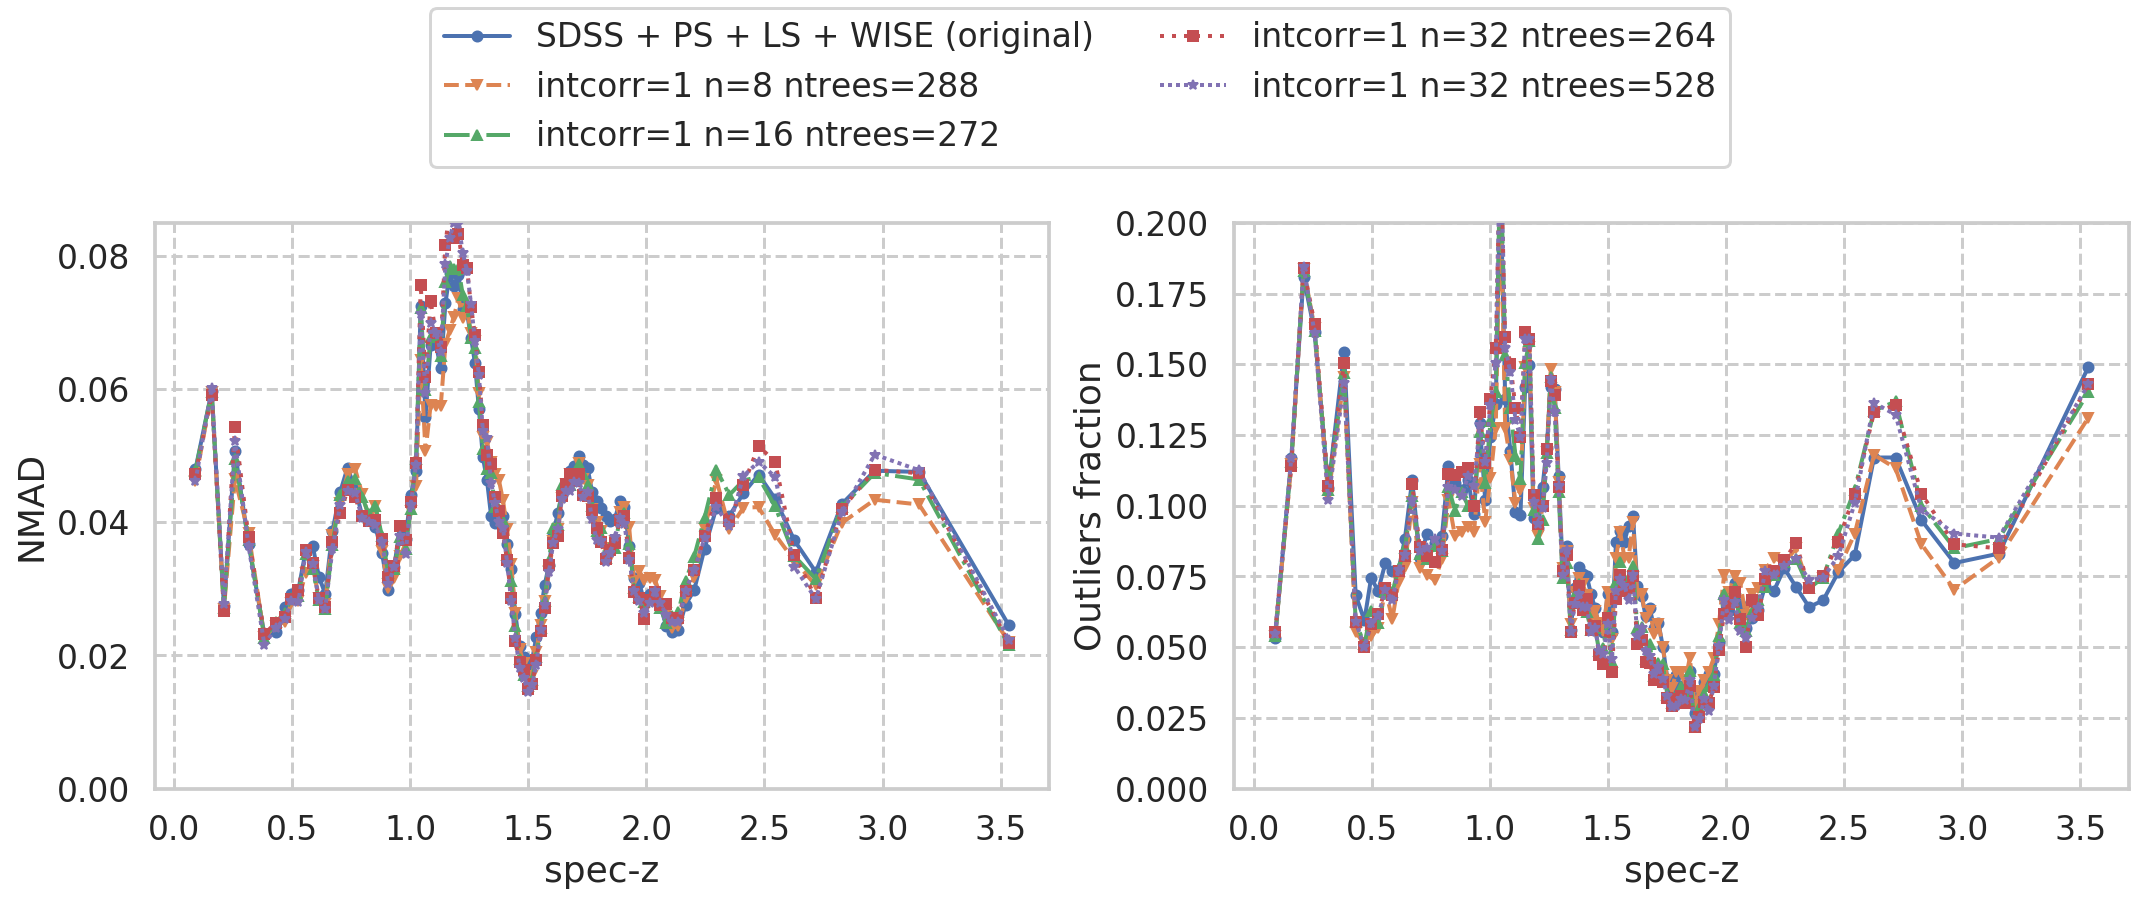
\includegraphics[width=\linewidth]{images/perturbations-n-35-zspec.png}
    \caption{SDSS + PanSTARRS + DESI LIS + WISE model with different number of perturbations comparison comparison on DR16 quasars by spec-z bins.}
    \label{fig:perturbations_n_35_zspec}
\end{figure*}

\begin{figure*}
    \centering
    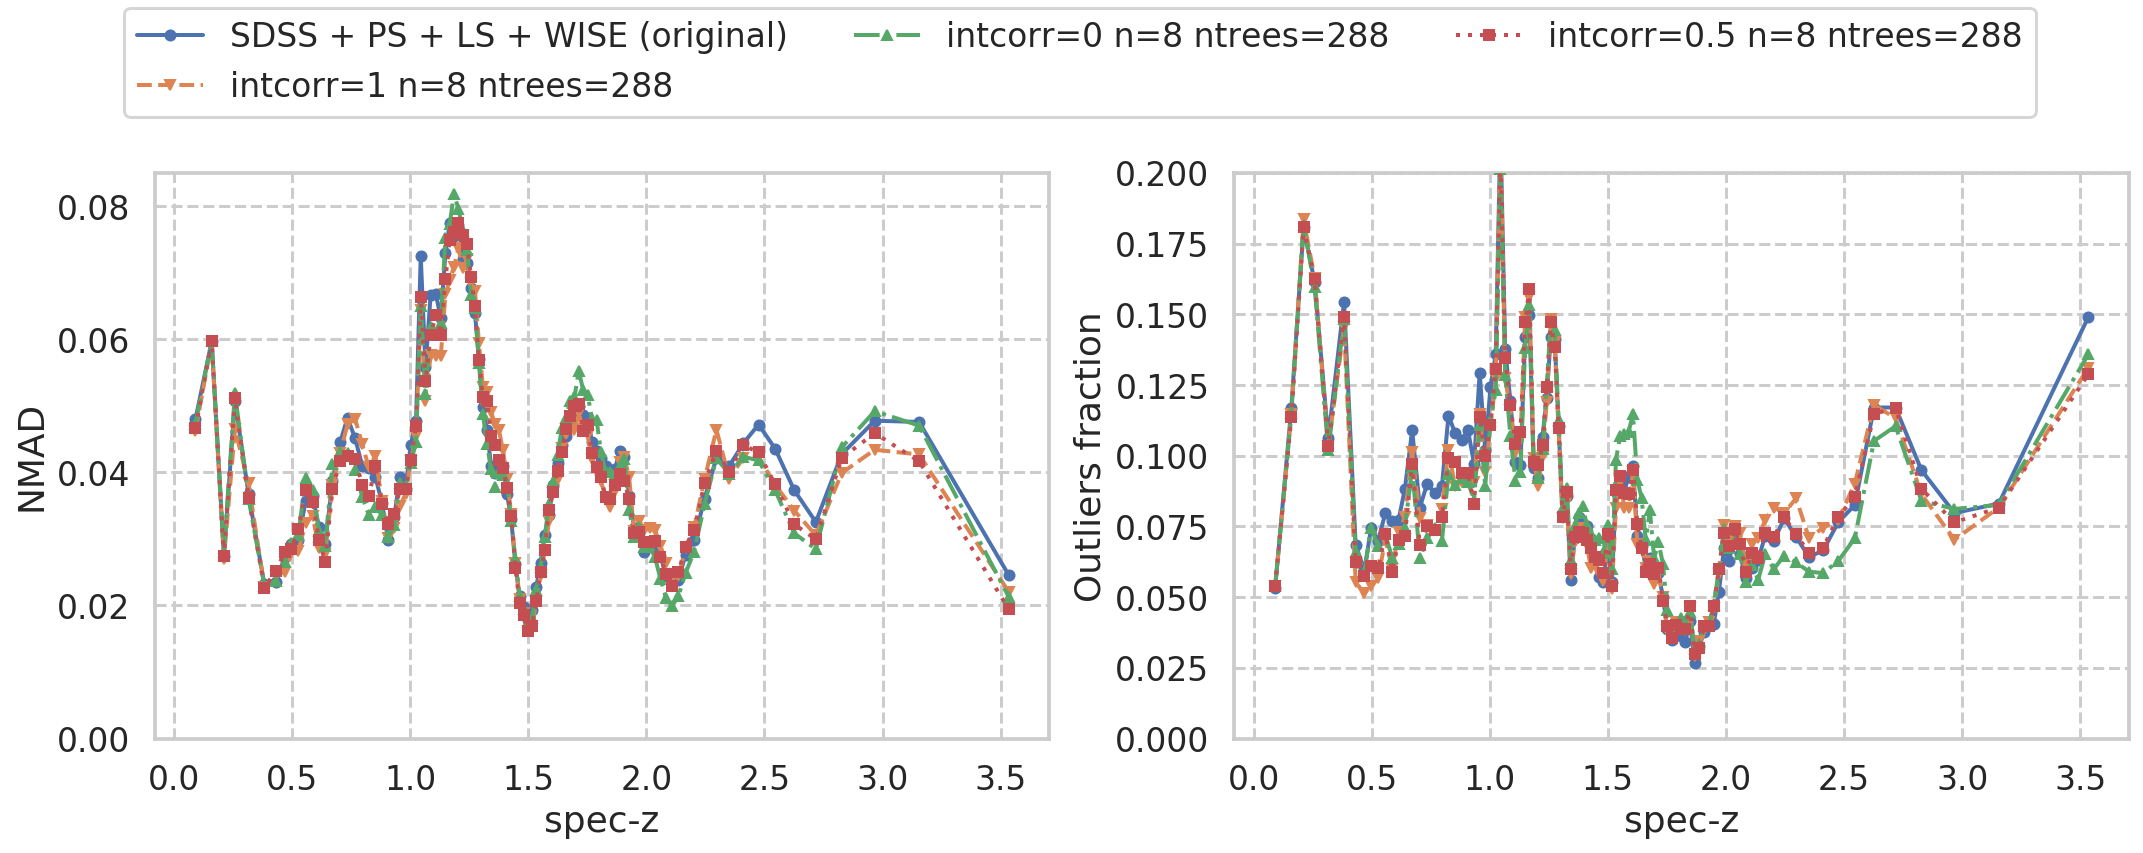
\includegraphics[width=\linewidth]{images/perturbations-intcorr-35-zspec.png}
    \caption{SDSS + PanSTARRS + DESI LIS + WISE model with different number of perturbations comparison comparison on DR16 quasars by z mag bins.}
    \label{fig:perturbations_n_35_z}
\end{figure*}

\subsection{ebv}

Примерно так же, но про поглощение.

\begin{figure*}
    \centering
    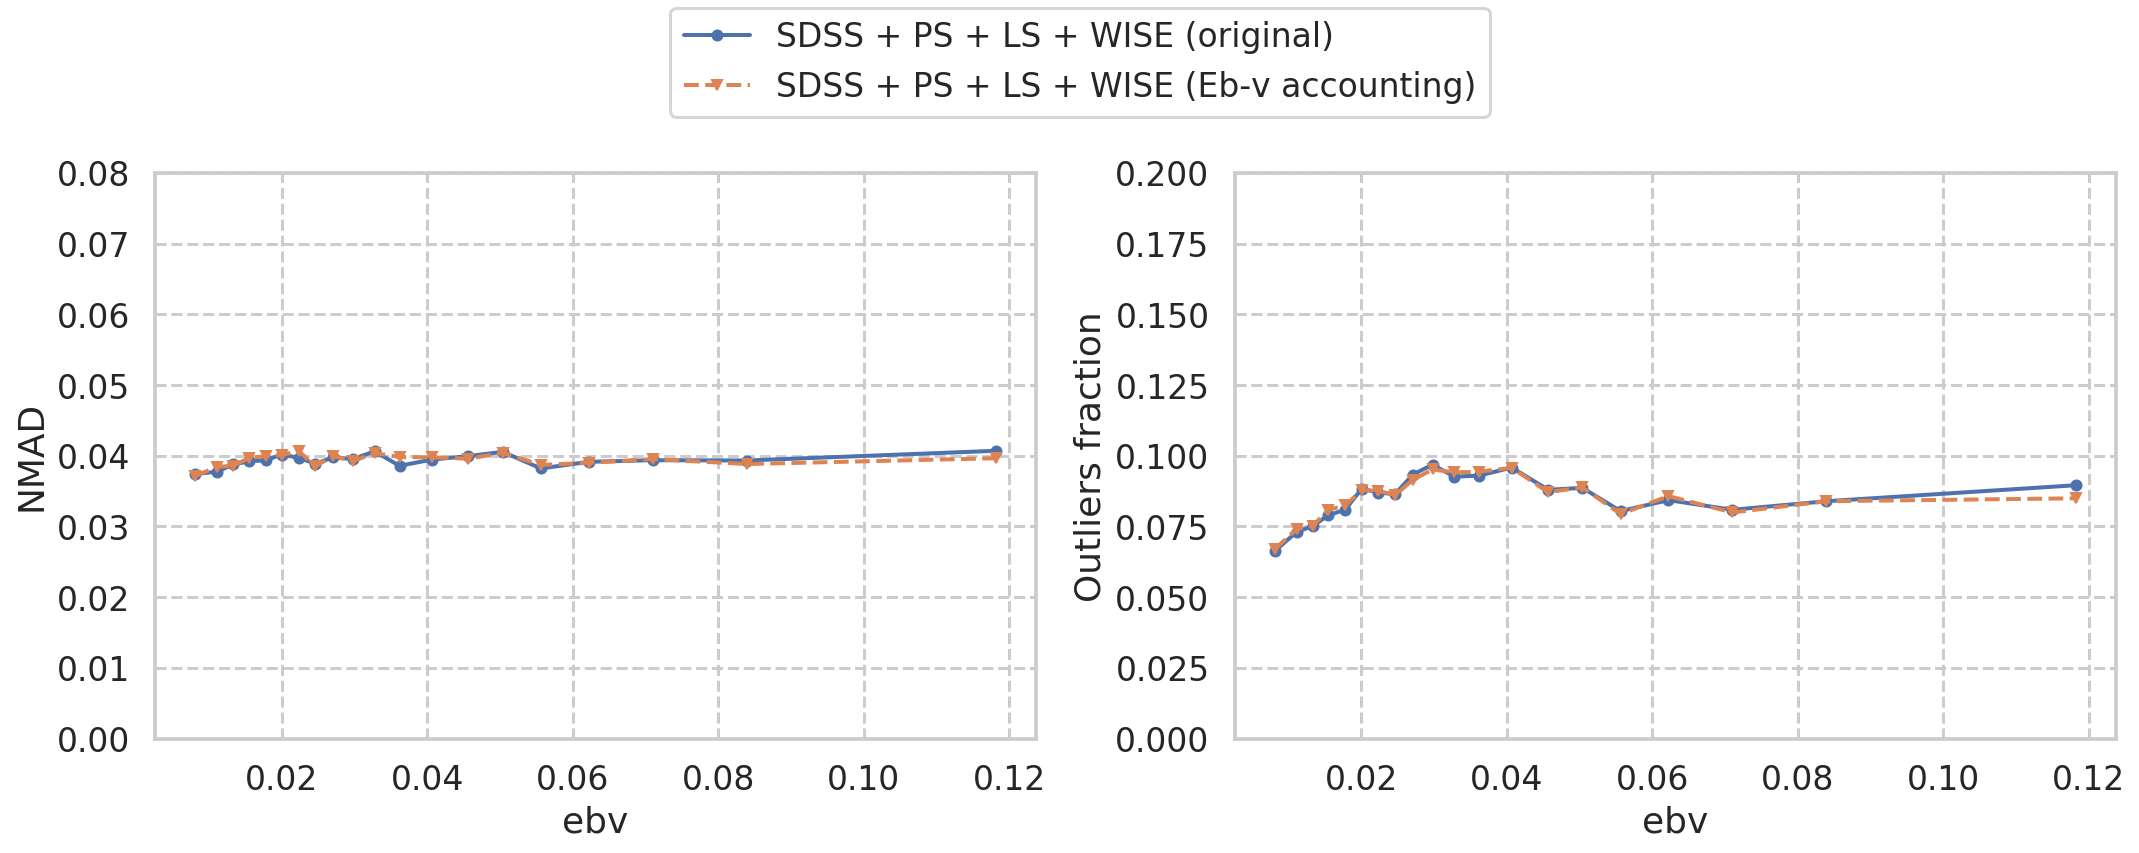
\includegraphics[width=\linewidth]{images/ebv-35-ebv.png}
    \caption{SDSS + PanSTARRS + DESI LIS + WISE models with and without ebv accounting comparison on DR16 quasars by spec-z bins.}
    \label{fig:ebv_35_zspec}
\end{figure*}

\begin{figure*}
    \centering
    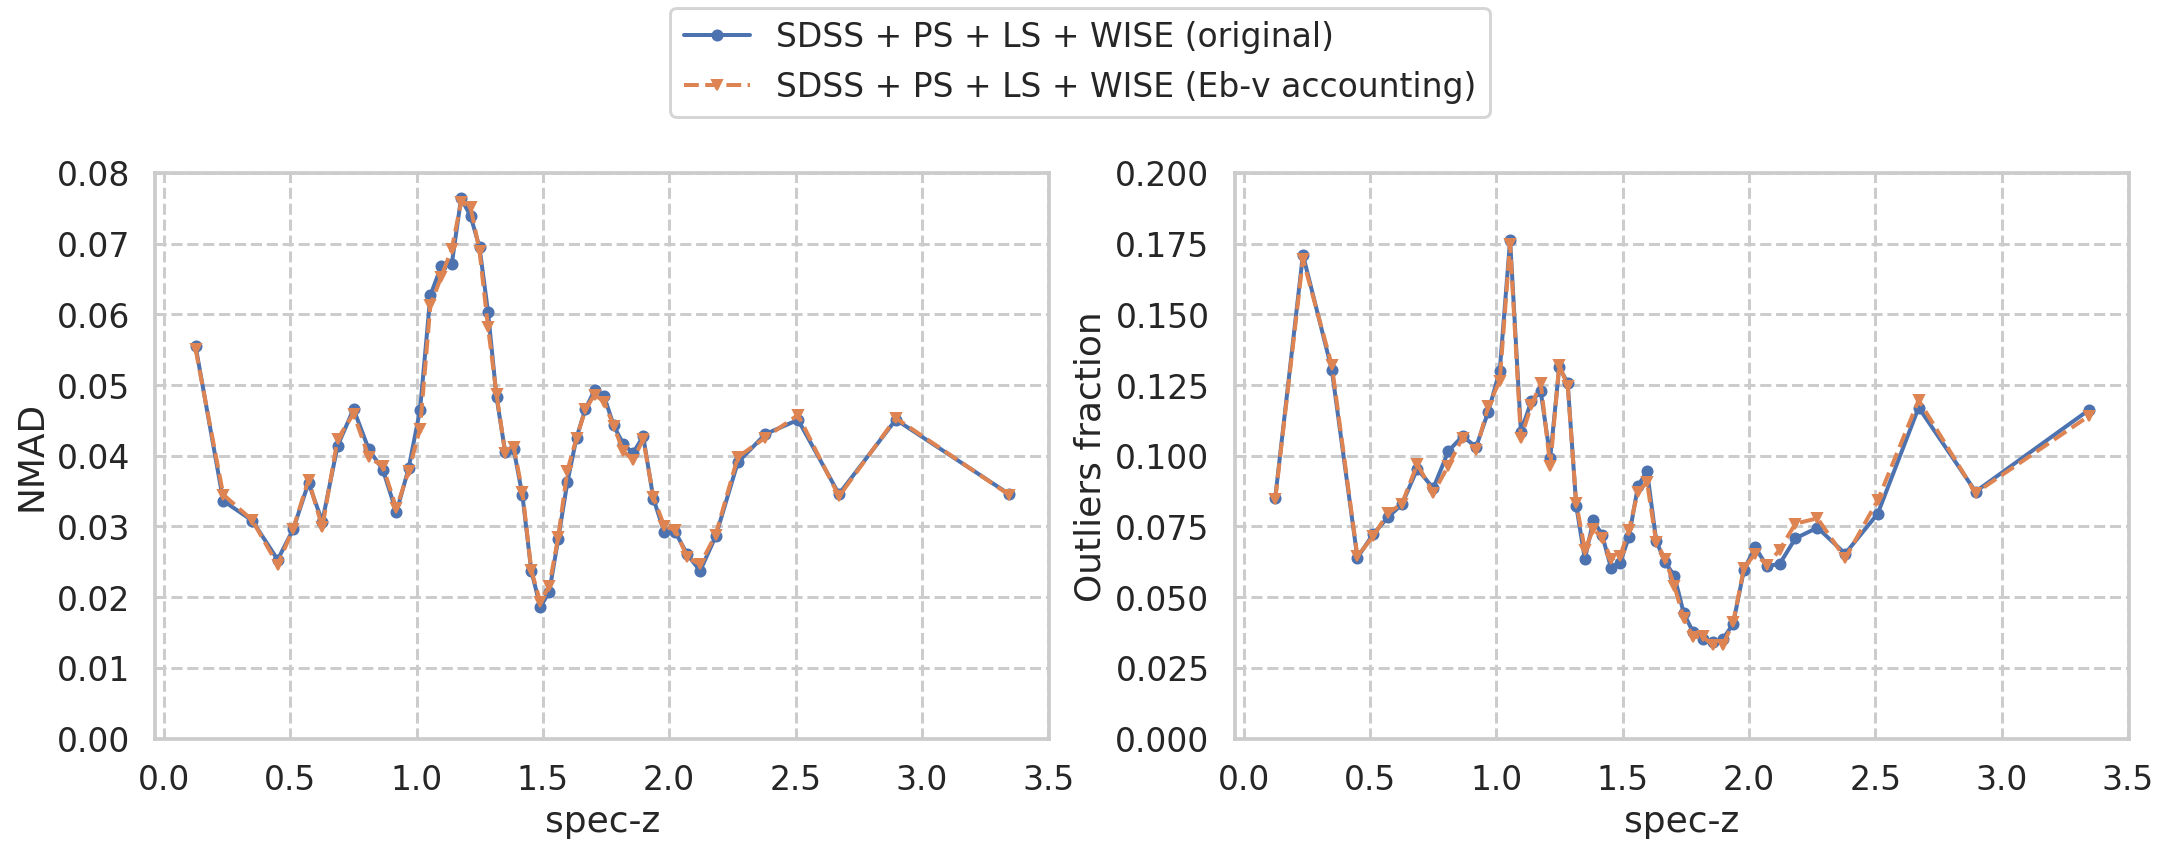
\includegraphics[width=\linewidth]{images/ebv-35-zspec.png}
    \caption{SDSS + PanSTARRS + DESI LIS + WISE models with and without ebv accounting comparison on DR16 quasars by ebv bins.}
    \label{fig:ebv_35_ebv}
\end{figure*}

\begin{figure*}
    \centering
    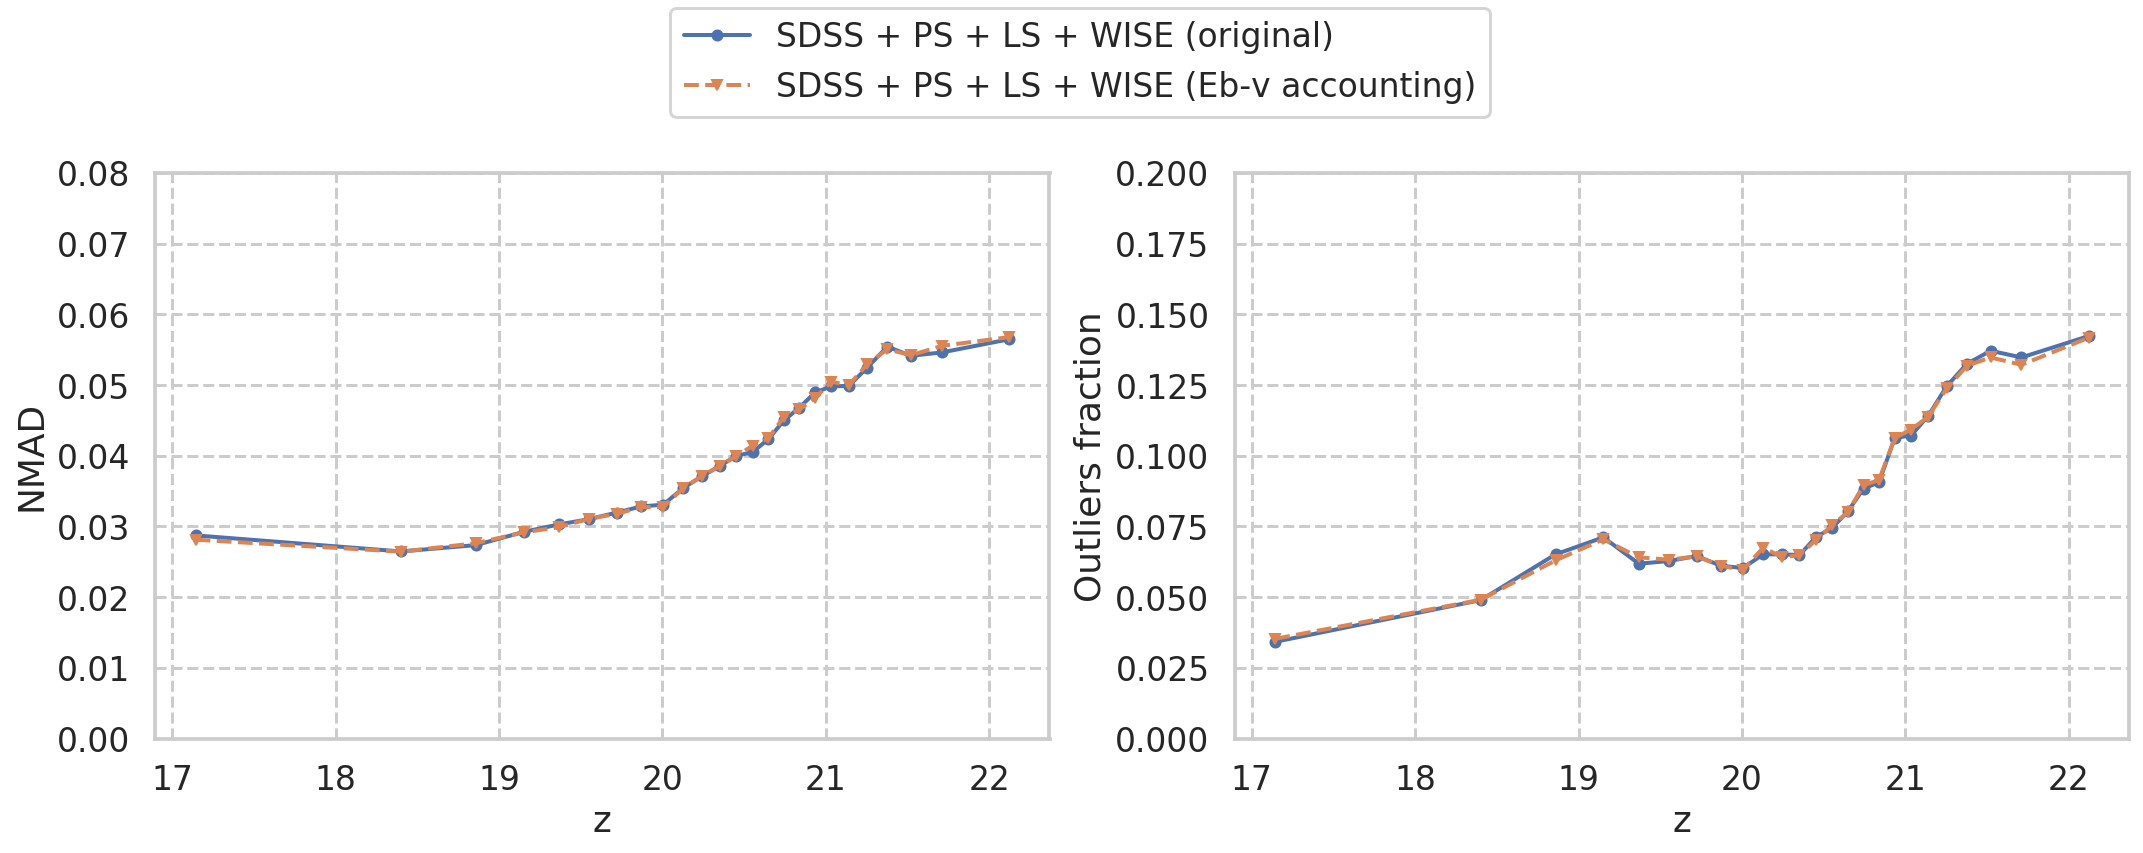
\includegraphics[width=\linewidth]{images/ebv-35-z.png}
    \caption{SDSS + PanSTARRS + DESI LIS + WISE models with and without ebv accounting comparison on DR16 quasars by z mag bins.}
    \label{fig:ebv_35_z}
\end{figure*}

\subsection{Best models detailed comparison}

\achtung{Эта часть самая важная. Её нужно продумать.}

\achtung{Сделать таблицы и графики, которые здесь хочется видеть. Тезисно изложить эту часть вместе с картинками}

\achtung{Тут рассказать про отдельно далекие/близкие, яркие/слабые, для 15!, (17?), 19!, (21?!), 22, 35!}

\subsubsection{Photo-z accuracy}

В таблице \ref{tab:metrics-s82x-a17-all30sec} приведены метрики... Видно, что лучшая из предложенных моделей превосходит модели SOTA в 2 раза по метрикам.

Сравнение на точечных и протяженных источниках.

Точность photo-z по метрикам NMAD, catout (каким еще?) на выборке 200 тыс. квазаров моделей 15, 17, 19, 21, 22, 35. Сравнение с Ananna, Brescia на Stripe82X.


Как лучше показывать метрики в бинах? Как в \ref{tab:metrics-by-rmag-s82x-a17} или графики, которые я построил недавно. 

Где-нибудь привести примеры спектров и прогнозов из "красной подложки". Думаю, это будет очень интересно. Описание паттернов ошибок? Тогда нужно добавить скаттерплоты на выборке квазаров.

Описать, что доля выбросов сильно растет на объектах с низким сигнал-шумом. При росте отношения сигнала к шуму точность растет.

Стоит описывать, что модели ведут себя неустойчиво в зависимости от spec-z?

\begin{figure*}
    \centering
    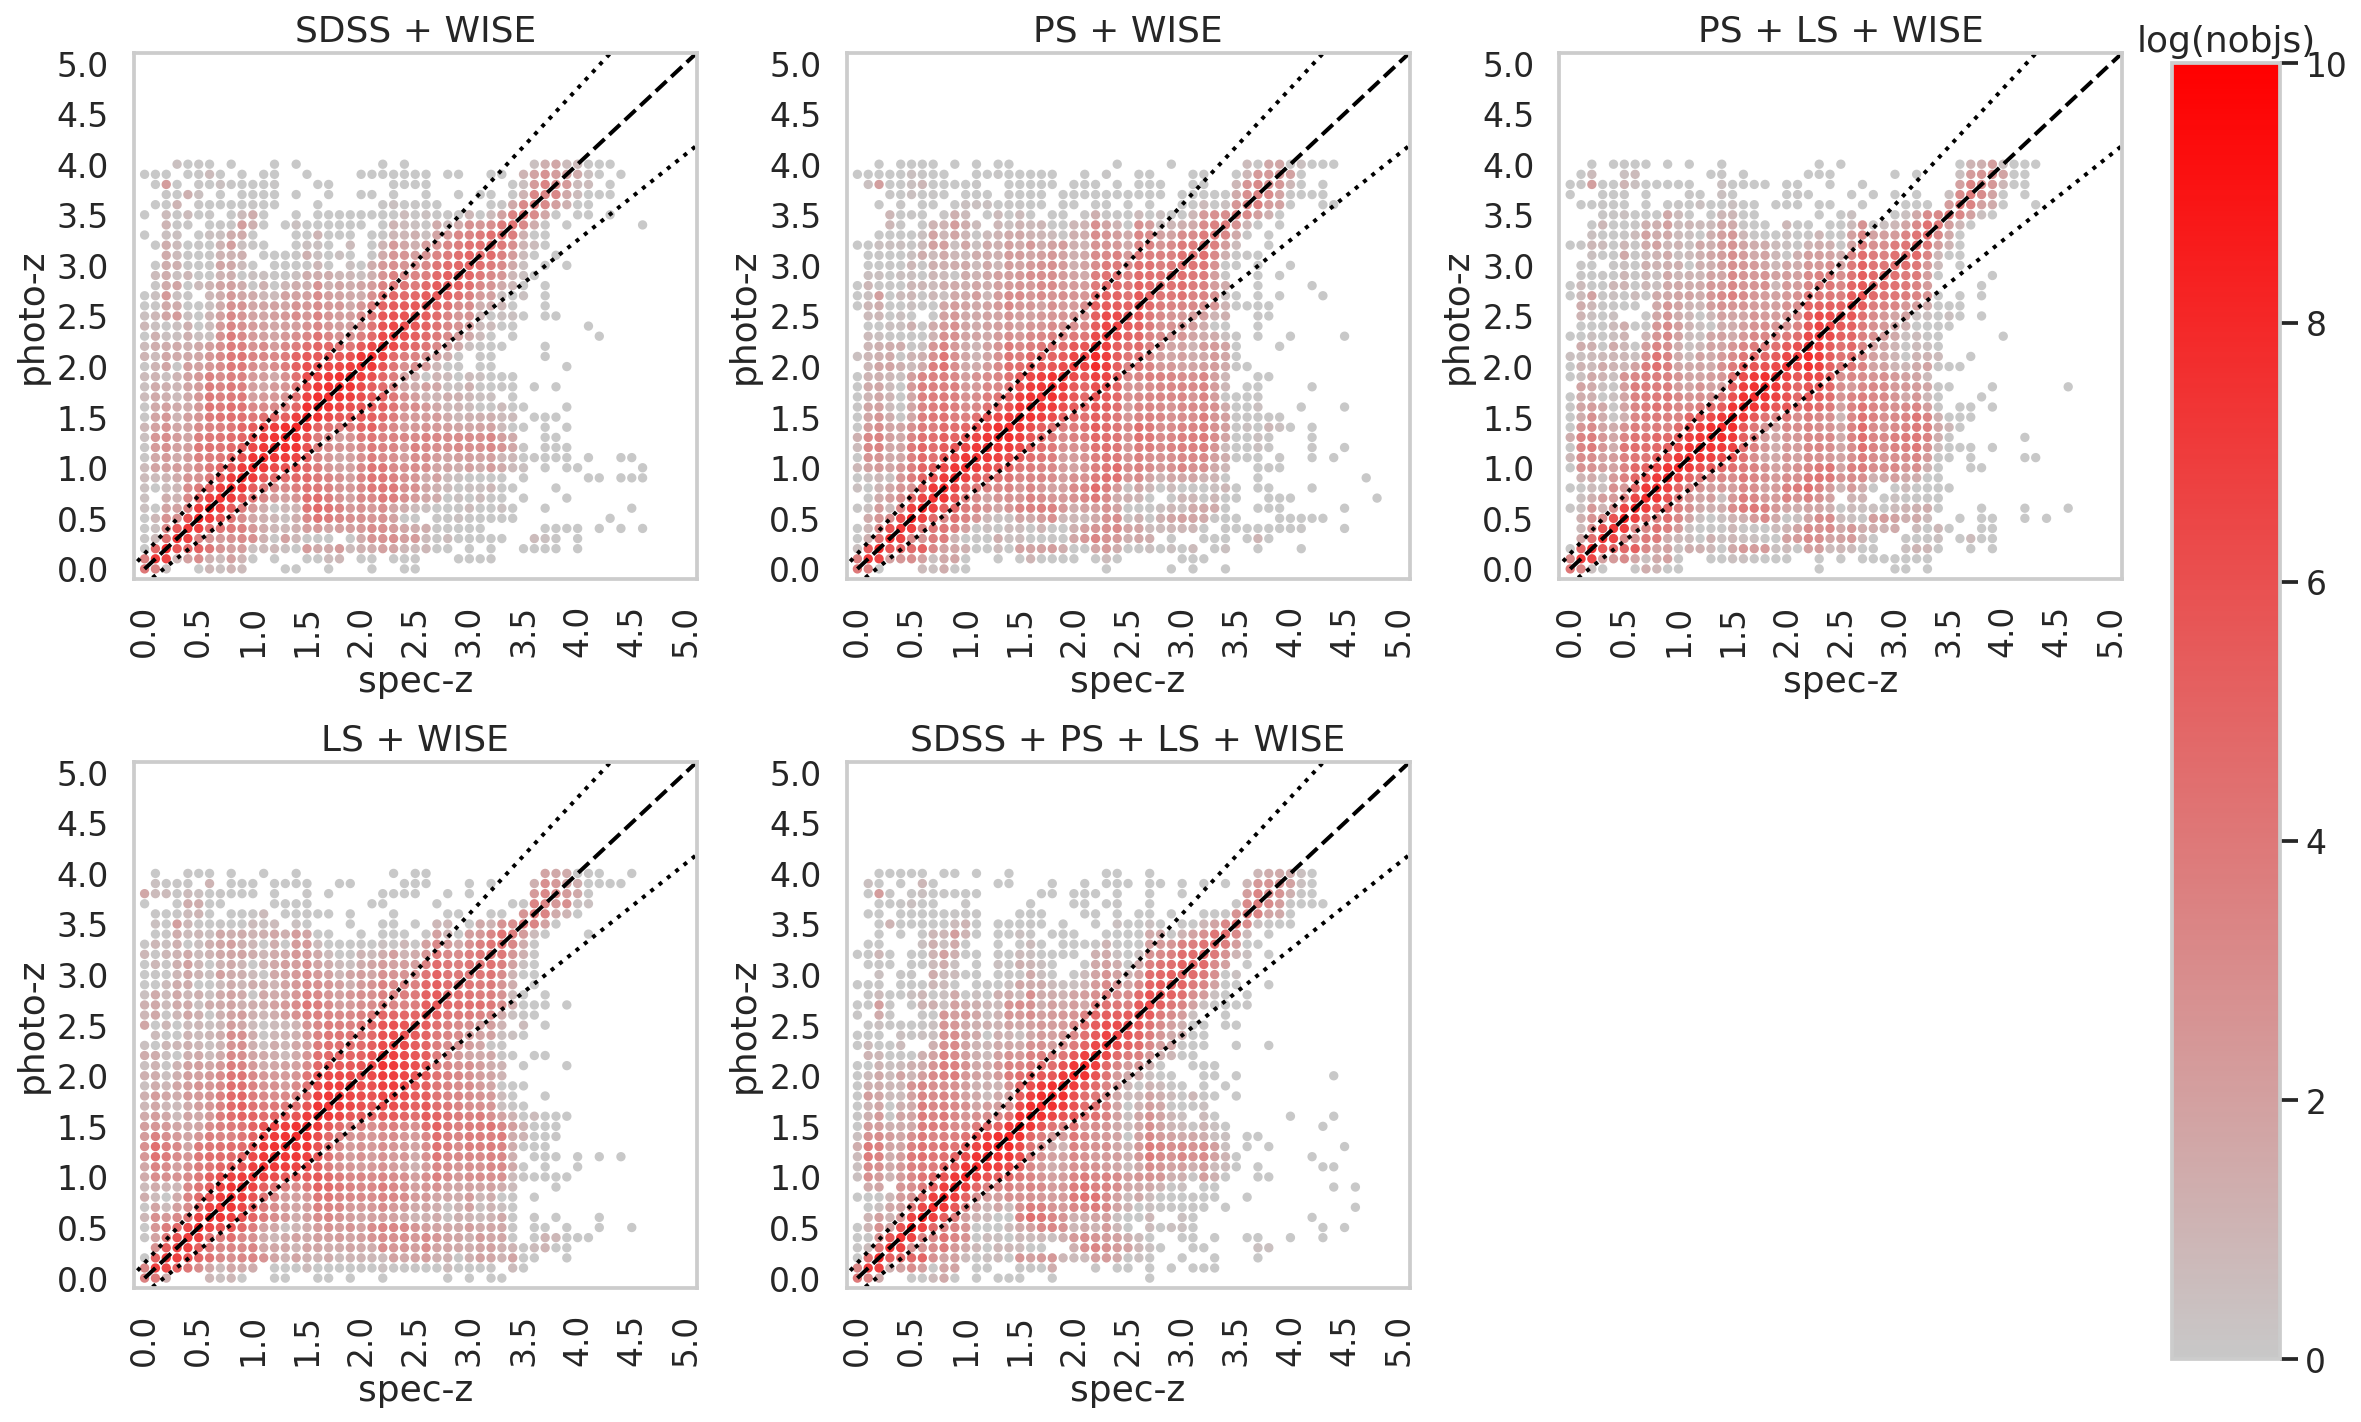
\includegraphics[width=\linewidth]{images/scatterplots-dr16qso.png}
    \caption{Scatterplots of catastrophic outliers on DR16 QSOs}
    \label{fig:my_label}
\end{figure*}

\begin{figure*}
    \centering
    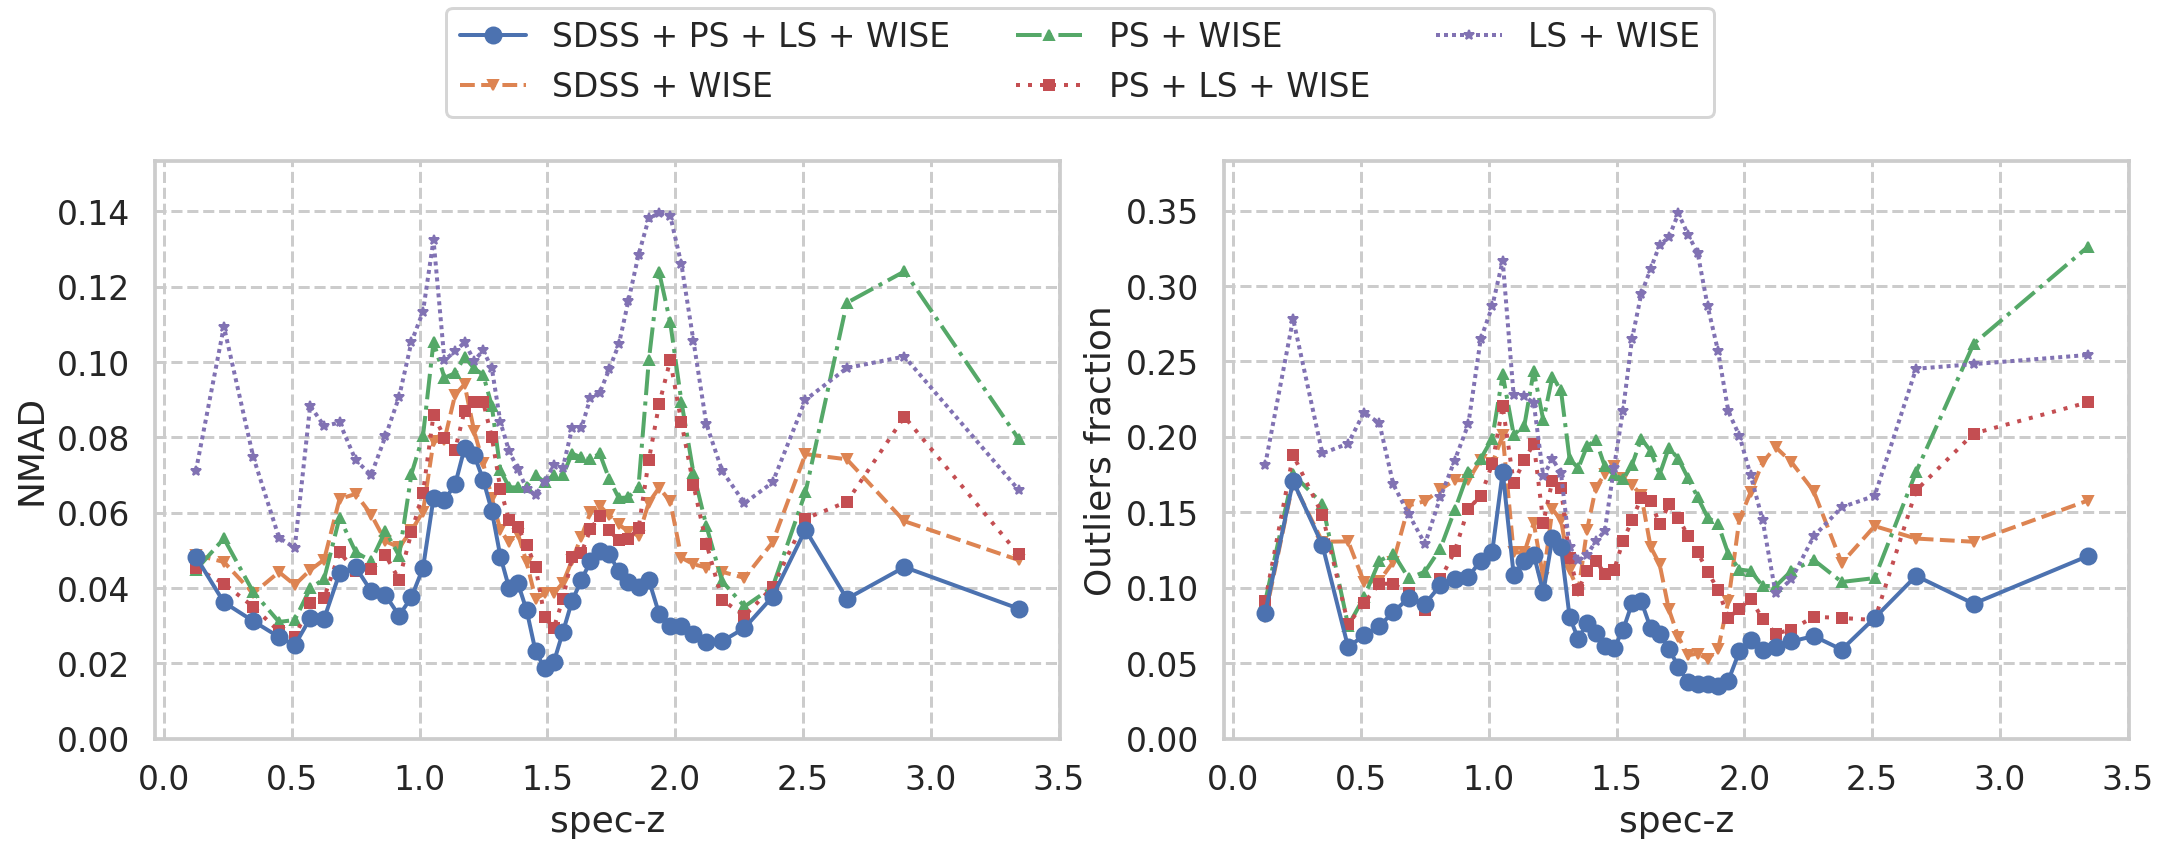
\includegraphics[width=\linewidth]{images/metrics-dr16qso-zspec.png}
    \caption{Метрики на квазарах DR16}
    \label{fig:my_label}
\end{figure*}

\begin{figure*}
    \centering
    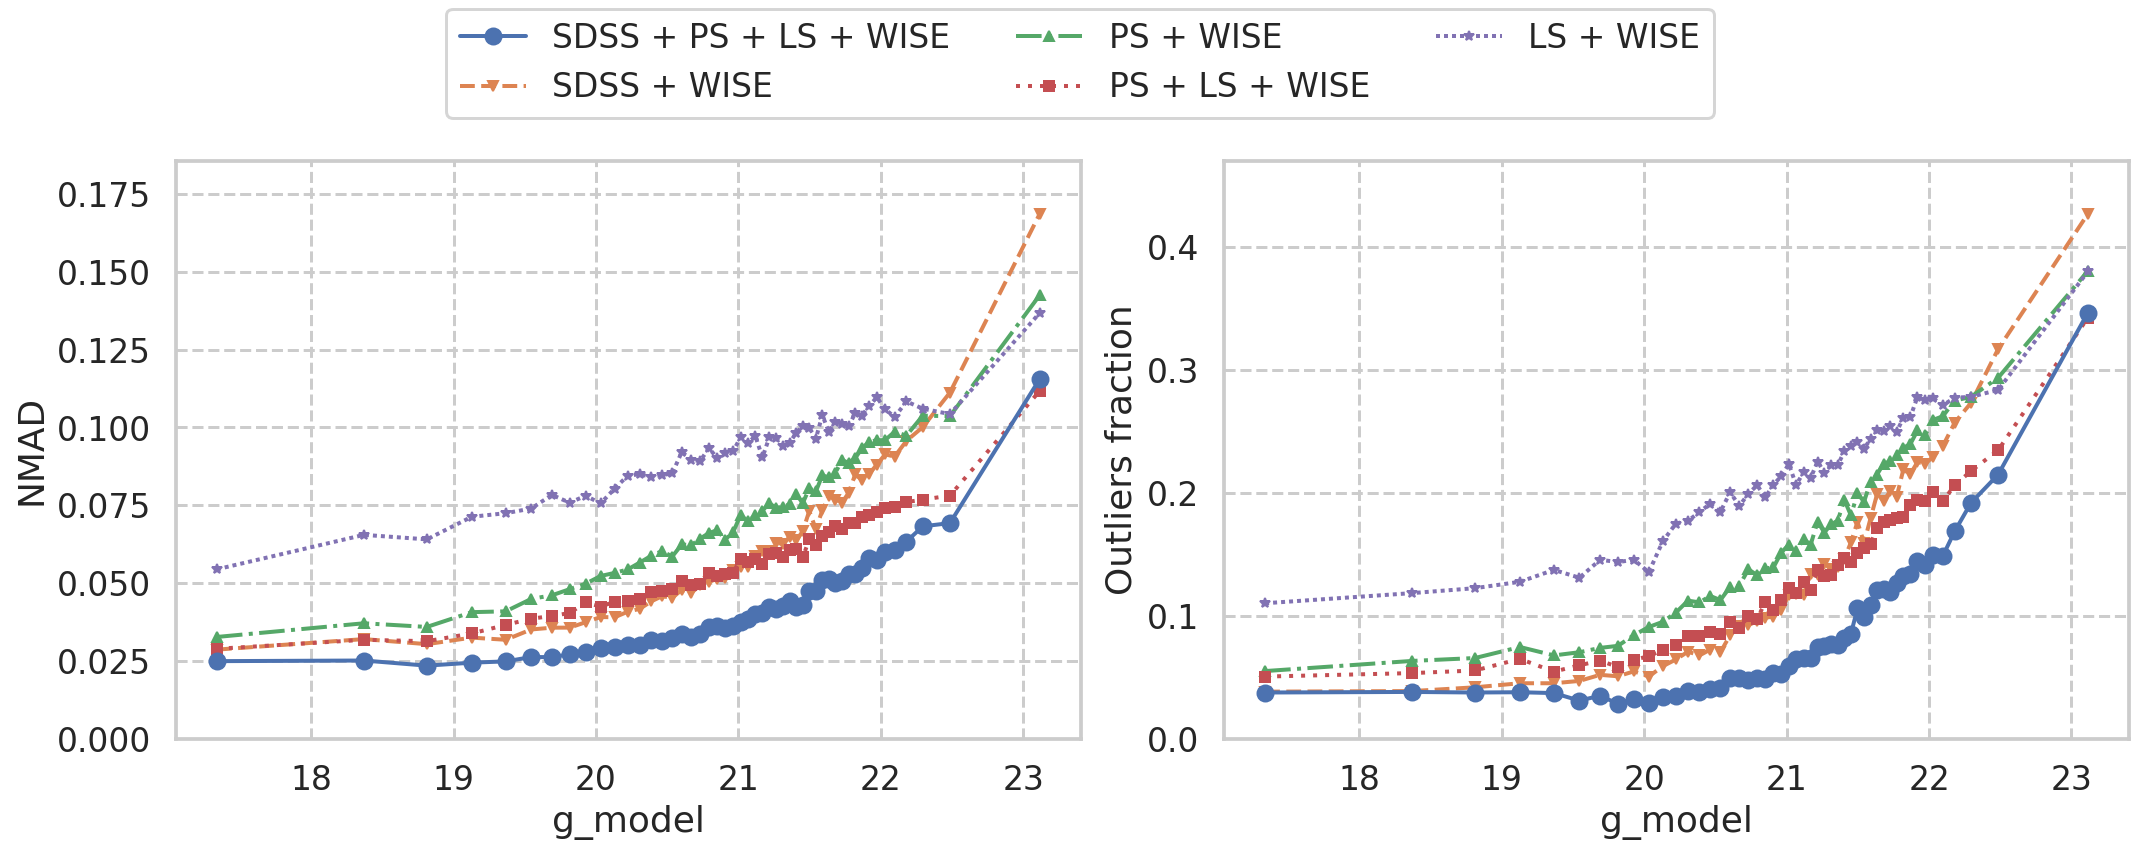
\includegraphics[width=\linewidth]{images/metrics-dr16qso-gmag.png}
    \caption{Метрики на квазарах DR16}
    \label{fig:metrics-dr16qso-gmag}
\end{figure*}

\begin{figure*}
    \centering
    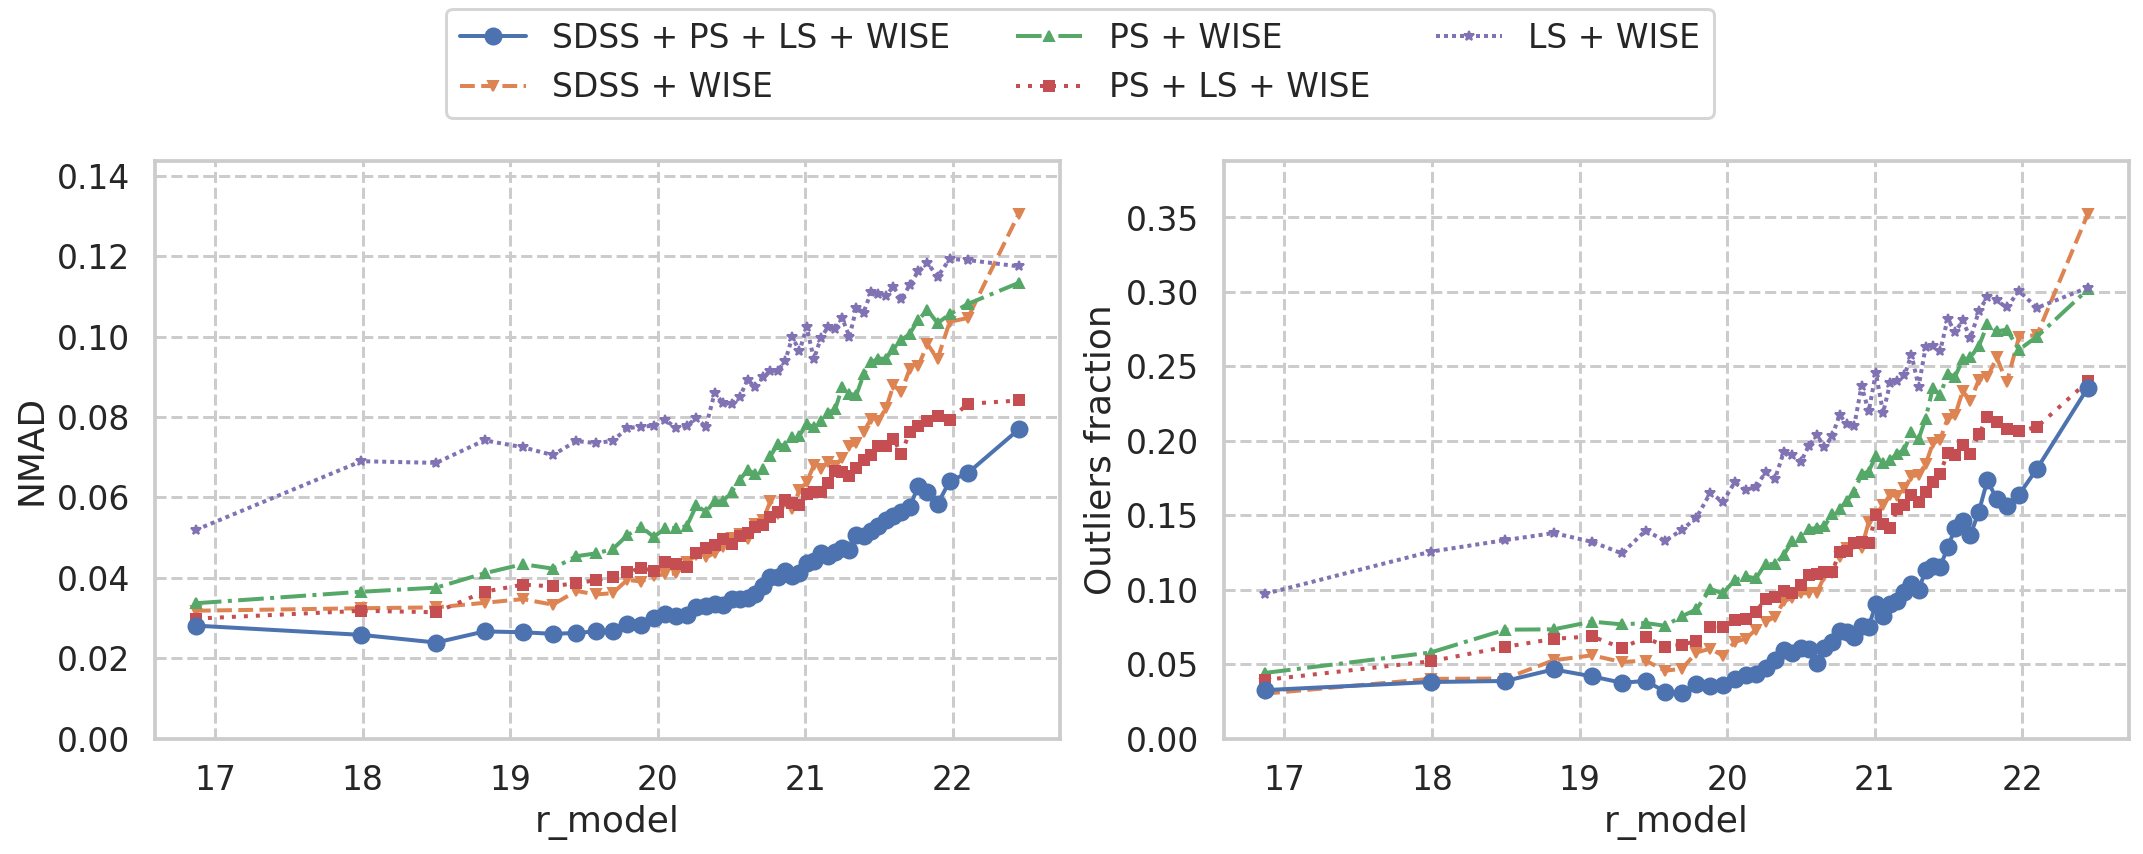
\includegraphics[width=\linewidth]{images/metrics-dr16qso-rmag.png}
    \caption{Метрики на квазарах DR16}
    \label{fig:metrics-dr16qso-sng}
\end{figure*}

\begin{figure*}
    \centering
    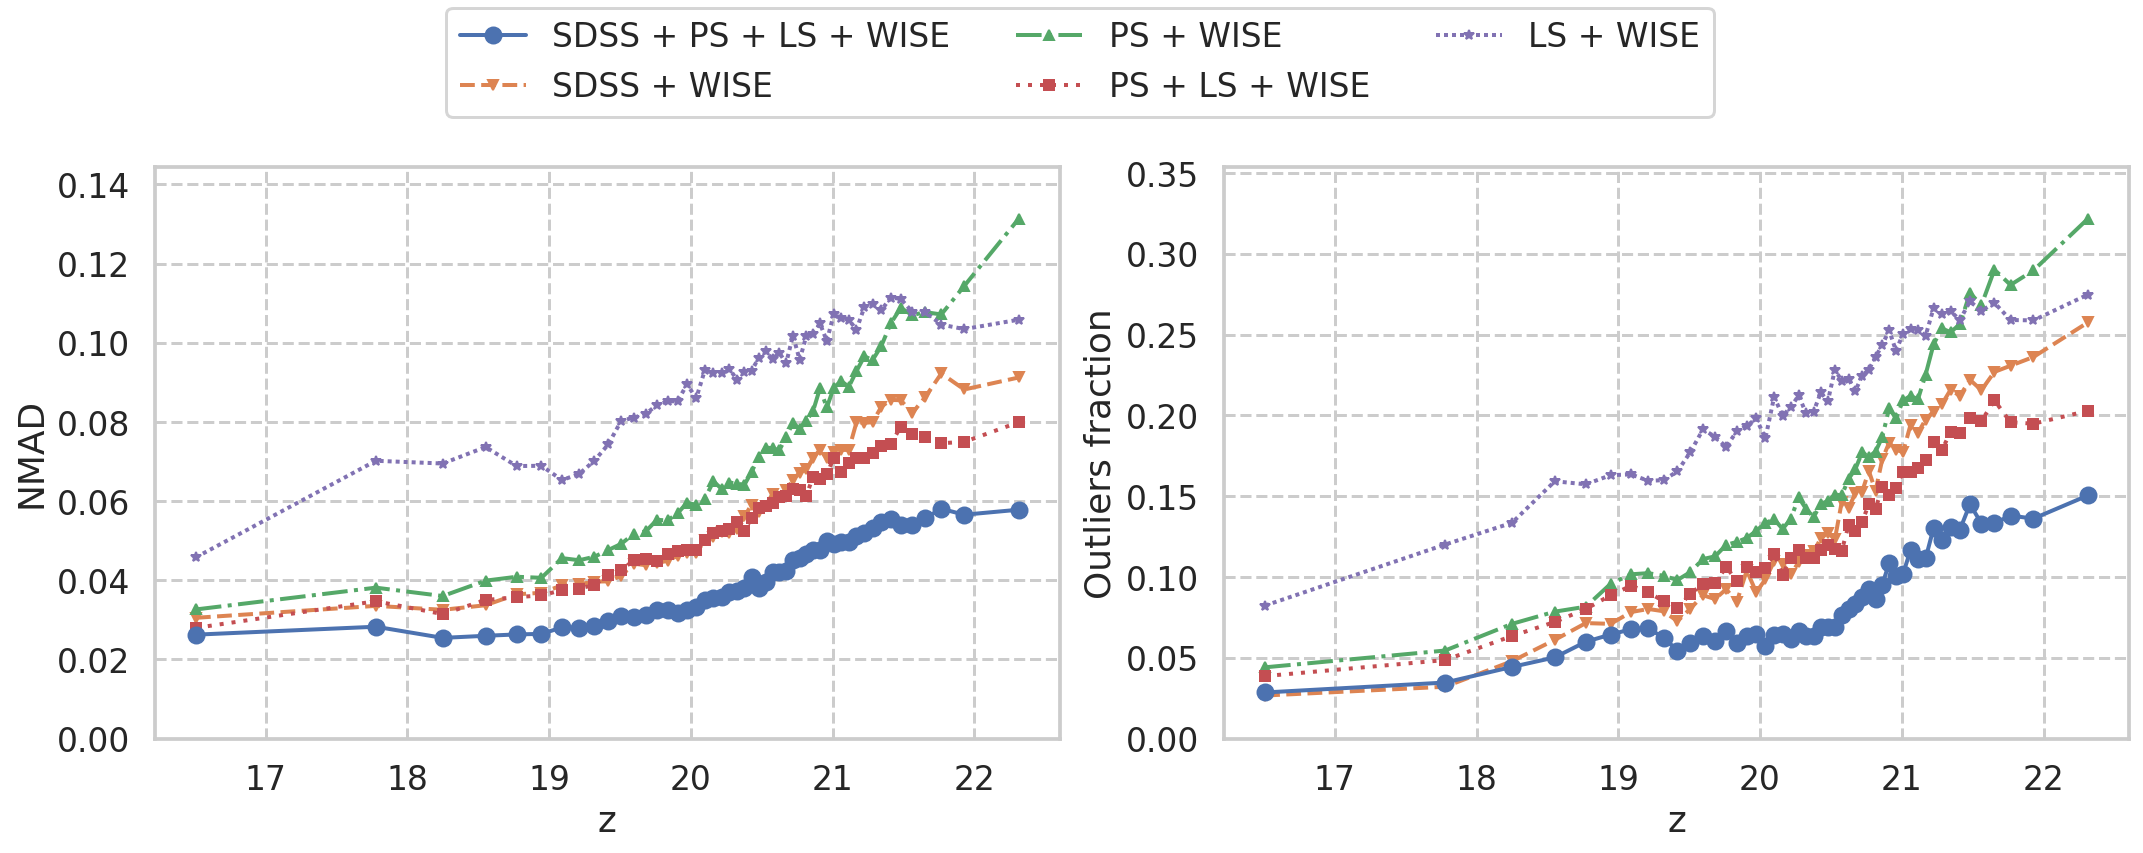
\includegraphics[width=\linewidth]{images/metrics-dr16qso-zmag.png}
    \caption{Метрики на квазарах DR16}
    \label{fig:metrics-dr16qso-snw1}
\end{figure*}

\begin{figure*}
    \centering
    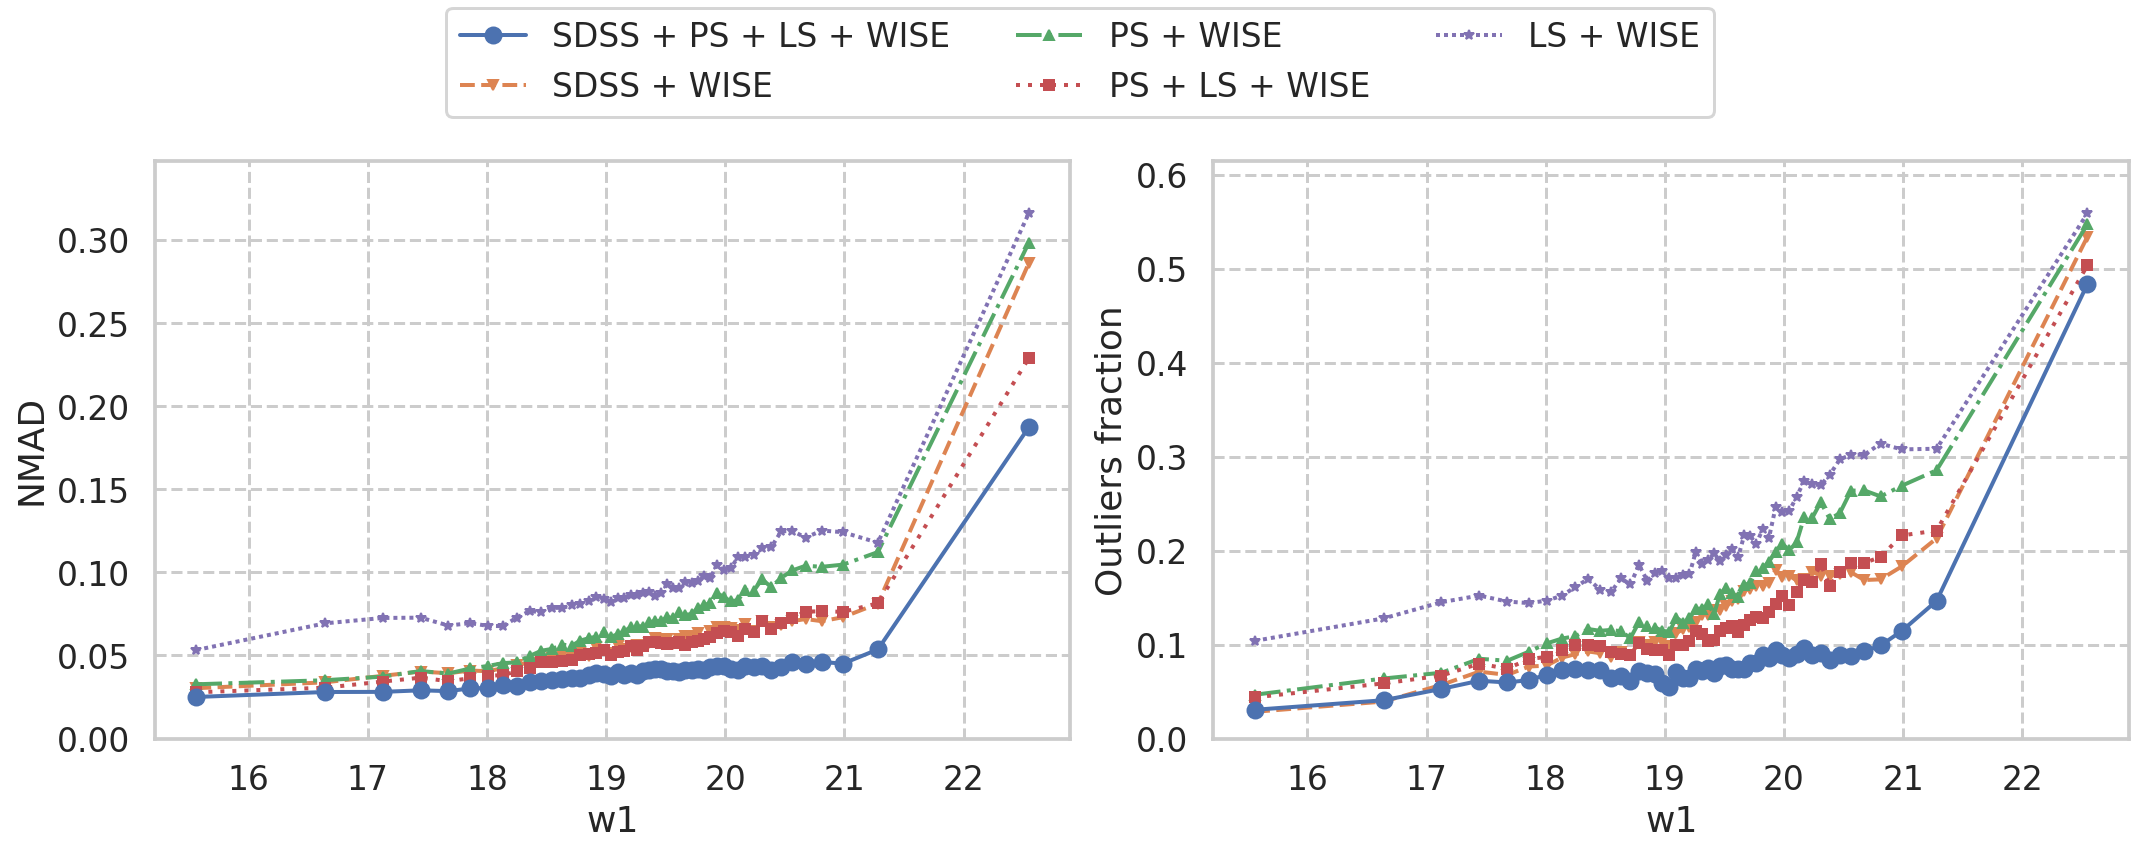
\includegraphics[width=\linewidth]{images/metrics-dr16qso-w1mag.png}
    \caption{Метрики на квазарах DR16}
    \label{fig:metrics-dr16qso-w1mag}
\end{figure*}

\begin{table*}
    \centering
    \begin{tabular}{lll}
    \hline
                        Model &   Dataset &                      All Objects \\
    \hline
                  SDSS + WISE &  S82X-A17 &                    0.049 / 0.127 \\
                  SDSS + WISE &  DR16 QSO &                    0.056 / 0.136 \\
                    PS + WISE &  S82X-A17 &                    0.059 / 0.153 \\
                    PS + WISE &  DR16 QSO &                    0.067 / 0.165 \\
                    LS + WISE &  S82X-A17 &                    0.076 / 0.177 \\
                    LS + WISE &  DR16 QSO &                    0.090 / 0.212 \\
        SDSS + PS + LS + WISE &  S82X-A17 &  \textbf{0.034} / \textbf{0.080} \\
        SDSS + PS + LS + WISE &  DR16 QSO &  \textbf{0.039} / \textbf{0.084} \\
     Templates (Ananna, 2017) &  S82X-A17 &                    0.065 / 0.170 \\
          ANN (Brescia, 2019) &  S82X-A17 &                    0.066 / 0.156 \\
                        nobjs &  S82X-A17 &                             2664 \\
                        nobjs &  DR16 QSO &                           211903 \\
    \hline
    \end{tabular}
    
    \caption{Метрики предложенных моделей и SOTA на тестовых выборках}
    \label{tab:metrics-rmag}
\end{table*}


\begin{table*}
    \centering
    \begin{tabular}{lllllll}
    \hline
                        Model &   Dataset &                         r < 19.5 &                  19.5 < r < 20.5 &                    20.5 < r < 21 &                    21 < r < 21.5 &                    21.5 < r < 23 \\
    \hline
                  SDSS + WISE &  S82X-A17 &                    0.028 / 0.031 &                    0.040 / 0.045 &                    0.058 / 0.115 &                    0.069 / 0.191 &                    0.098 / 0.285 \\
                  SDSS + WISE &  DR16 QSO &                    0.033 / 0.046 &                    0.042 / 0.069 &                    0.056 / 0.119 &                    0.071 / 0.177 &                    0.095 / 0.252 \\
                    PS + WISE &  S82X-A17 &                    0.031 / 0.046 &                    0.049 / 0.083 &                    0.063 / 0.138 &                    0.086 / 0.210 &                    0.107 / 0.313 \\
                    PS + WISE &  DR16 QSO &                    0.040 / 0.069 &                    0.053 / 0.105 &                    0.069 / 0.157 &                    0.085 / 0.206 &                    0.103 / 0.267 \\
                    LS + WISE &  S82X-A17 &                    0.050 / 0.069 &                    0.076 / 0.150 &                    0.078 / 0.182 &                    0.082 / 0.184 &                    0.109 / 0.303 \\
                    LS + WISE &  DR16 QSO &                    0.068 / 0.127 &                    0.079 / 0.166 &                    0.091 / 0.211 &                    0.103 / 0.249 &                    0.115 / 0.288 \\
        SDSS + PS + LS + WISE &  S82X-A17 &  \textbf{0.023} / \textbf{0.027} &  \textbf{0.028} / \textbf{0.031} &  \textbf{0.038} / \textbf{0.057} &  \textbf{0.044} / \textbf{0.116} &  \textbf{0.064} / \textbf{0.181} \\
        SDSS + PS + LS + WISE &  DR16 QSO &  \textbf{0.026} / \textbf{0.039} &  \textbf{0.030} / \textbf{0.043} &  \textbf{0.038} / \textbf{0.067} &  \textbf{0.048} / \textbf{0.102} &  \textbf{0.060} / \textbf{0.163} \\
     Templates (Ananna, 2017) &  S82X-A17 &                    0.061 / 0.099 &                    0.061 / 0.137 &                    0.061 / 0.170 &                    0.069 / 0.219 &                    0.082 / 0.247 \\
          ANN (Brescia, 2019) &  S82X-A17 &                    0.062 / 0.102 &                    0.057 / 0.125 &                    0.060 / 0.140 &                    0.073 / 0.209 &                    0.084 / 0.222 \\
                        nobjs &  S82X-A17 &                              586 &                              686 &                              407 &                              398 &                              576 \\
                        nobjs &  DR16 QSO &                            29085 &                            53555 &                            41596 &                            43574 &                            43934 \\
    \hline
    \end{tabular}
    
    \caption{Метрики предложенных моделей и SOTA на тестовых выборках в бинах по r}
    \label{tab:metrics-rmag}
\end{table*}


\begin{table*}
    \centering
    \begin{tabular}{lllllll}
    \hline
                        Model &   Dataset &                           g < 20 &                      20 < g < 21 &                    21 < g < 21.5 &                    21.5 < g < 22 &                      22 < g < 24 \\
    \hline
                  SDSS + WISE &  S82X-A17 &                    0.027 / 0.028 &                    0.042 / 0.062 &                    0.061 / 0.122 &                    0.063 / 0.170 &                    0.108 / 0.299 \\
                  SDSS + WISE &  DR16 QSO &                    0.033 / 0.046 &                    0.046 / 0.081 &                    0.062 / 0.137 &                    0.078 / 0.200 &                    0.104 / 0.289 \\
                    PS + WISE &  S82X-A17 &                    0.032 / 0.046 &                    0.050 / 0.110 &                    0.060 / 0.144 &                    0.082 / 0.221 &                    0.099 / 0.295 \\
                    PS + WISE &  DR16 QSO &                    0.042 / 0.070 &                    0.061 / 0.122 &                    0.074 / 0.172 &                    0.088 / 0.226 &                    0.104 / 0.290 \\
                    LS + WISE &  S82X-A17 &                    0.054 / 0.083 &                    0.078 / 0.173 &                    0.078 / 0.183 &                    0.083 / 0.171 &                    0.099 / 0.285 \\
                    LS + WISE &  DR16 QSO &                    0.070 / 0.131 &                    0.087 / 0.188 &                    0.096 / 0.223 &                    0.102 / 0.255 &                    0.109 / 0.293 \\
        SDSS + PS + LS + WISE &  S82X-A17 &  \textbf{0.021} / \textbf{0.020} &  \textbf{0.030} / \textbf{0.046} &  \textbf{0.035} / \textbf{0.058} &  \textbf{0.043} / \textbf{0.095} &  \textbf{0.073} / \textbf{0.198} \\
        SDSS + PS + LS + WISE &  DR16 QSO &  \textbf{0.026} / \textbf{0.035} &  \textbf{0.033} / \textbf{0.044} &  \textbf{0.042} / \textbf{0.075} &  \textbf{0.053} / \textbf{0.124} &  \textbf{0.068} / \textbf{0.201} \\
     Templates (Ananna, 2017) &  S82X-A17 &                    0.061 / 0.110 &                    0.058 / 0.135 &                    0.068 / 0.192 &                    0.071 / 0.206 &                    0.085 / 0.246 \\
          ANN (Brescia, 2019) &  S82X-A17 &                    0.062 / 0.115 &                    0.055 / 0.119 &                    0.069 / 0.159 &                    0.075 / 0.187 &                    0.083 / 0.231 \\
                        nobjs &  S82X-A17 &                              609 &                              725 &                              433 &                              359 &                              529 \\
                        nobjs &  DR16 QSO &                            38951 &                            59379 &                            43883 &                            44277 &                            25123 \\
    \hline
    \end{tabular}
    
    \caption{Метрики предложенных моделей и SOTA на тестовых выборках в бинах по g}
    \label{tab:metrics-rmag}
\end{table*}


\begin{table*}
    \centering
    \begin{tabular}{lllllll}
    \hline
                        Model &   Dataset &                           z < 19 &                      19 < z < 20 &                    20 < z < 20.5 &                    20.5 < z < 21 &                      21 < z < 23 \\
    \hline
                  SDSS + WISE &  S82X-A17 &                    0.030 / 0.029 &                    0.040 / 0.060 &                    0.050 / 0.098 &                    0.065 / 0.176 &                    0.099 / 0.284 \\
                  SDSS + WISE &  DR16 QSO &                    0.034 / 0.051 &                    0.042 / 0.085 &                    0.053 / 0.112 &                    0.066 / 0.157 &                    0.082 / 0.214 \\
                    PS + WISE &  S82X-A17 &                    0.031 / 0.044 &                    0.046 / 0.077 &                    0.063 / 0.123 &                    0.079 / 0.199 &                    0.119 / 0.335 \\
                    PS + WISE &  DR16 QSO &                    0.038 / 0.070 &                    0.051 / 0.111 &                    0.064 / 0.139 &                    0.079 / 0.176 &                    0.102 / 0.257 \\
                    LS + WISE &  S82X-A17 &                    0.046 / 0.067 &                    0.075 / 0.134 &                    0.077 / 0.187 &                    0.084 / 0.199 &                    0.109 / 0.305 \\
                    LS + WISE &  DR16 QSO &                    0.065 / 0.135 &                    0.078 / 0.179 &                    0.092 / 0.205 &                    0.099 / 0.232 &                    0.107 / 0.261 \\
        SDSS + PS + LS + WISE &  S82X-A17 &  \textbf{0.023} / \textbf{0.027} &  \textbf{0.028} / \textbf{0.036} &  \textbf{0.035} / \textbf{0.071} &  \textbf{0.040} / \textbf{0.086} &  \textbf{0.060} / \textbf{0.182} \\
        SDSS + PS + LS + WISE &  DR16 QSO &  \textbf{0.026} / \textbf{0.047} &  \textbf{0.030} / \textbf{0.063} &  \textbf{0.037} / \textbf{0.064} &  \textbf{0.045} / \textbf{0.088} &  \textbf{0.054} / \textbf{0.129} \\
     Templates (Ananna, 2017) &  S82X-A17 &                    0.063 / 0.091 &                    0.062 / 0.146 &                    0.058 / 0.145 &                    0.061 / 0.186 &                    0.085 / 0.279 \\
          ANN (Brescia, 2019) &  S82X-A17 &                    0.063 / 0.091 &                    0.059 / 0.137 &                    0.056 / 0.127 &                    0.063 / 0.159 &                    0.090 / 0.257 \\
                        nobjs &  S82X-A17 &                              552 &                              665 &                              440 &                              408 &                              587 \\
                        nobjs &  DR16 QSO &                            24762 &                            46885 &                            38244 &                            44079 &                            57843 \\
    \hline
    \end{tabular}
    
    \caption{Метрики предложенных моделей и SOTA на тестовых выборках в бинах по z}
    \label{tab:metrics-rmag}
\end{table*}


\begin{table*}
    \centering
    \begin{tabular}{lllllll}
    \hline
                        Model &   Dataset &                        w1 < 18.5 &                   18.5 < w1 < 19 &                   19 < w1 < 19.5 &                   19.5 < w1 < 20 &                   20 < w1 < 22.5 \\
    \hline
                  SDSS + WISE &  S82X-A17 &                    0.034 / 0.039 &                    0.047 / 0.093 &                    0.060 / 0.149 &                    0.067 / 0.201 &                    0.080 / 0.251 \\
                  SDSS + WISE &  DR16 QSO &                    0.040 / 0.071 &                    0.051 / 0.096 &                    0.056 / 0.123 &                    0.062 / 0.160 &                    0.072 / 0.189 \\
                    PS + WISE &  S82X-A17 &                    0.036 / 0.062 &                    0.054 / 0.080 &                    0.070 / 0.149 &                    0.093 / 0.223 &                    0.120 / 0.350 \\
                    PS + WISE &  DR16 QSO &                    0.042 / 0.090 &                    0.059 / 0.117 &                    0.067 / 0.133 &                    0.078 / 0.174 &                    0.098 / 0.254 \\
                    LS + WISE &  S82X-A17 &                    0.058 / 0.094 &                    0.070 / 0.130 &                    0.076 / 0.181 &                    0.093 / 0.226 &                    0.128 / 0.339 \\
                    LS + WISE &  DR16 QSO &                    0.069 / 0.146 &                    0.081 / 0.171 &                    0.086 / 0.184 &                    0.095 / 0.215 &                    0.118 / 0.293 \\
        SDSS + PS + LS + WISE &  S82X-A17 &  \textbf{0.026} / \textbf{0.031} &  \textbf{0.034} / \textbf{0.067} &  \textbf{0.039} / \textbf{0.079} &  \textbf{0.042} / \textbf{0.123} &  \textbf{0.046} / \textbf{0.150} \\
        SDSS + PS + LS + WISE &  DR16 QSO &  \textbf{0.030} / \textbf{0.061} &  \textbf{0.037} / \textbf{0.067} &  \textbf{0.040} / \textbf{0.069} &  \textbf{0.042} / \textbf{0.082} &  \textbf{0.045} / \textbf{0.109} \\
     Templates (Ananna, 2017) &  S82X-A17 &                    0.062 / 0.140 &                    0.072 / 0.161 &                    0.058 / 0.149 &                    0.072 / 0.216 &                    0.072 / 0.215 \\
          ANN (Brescia, 2019) &  S82X-A17 &                    0.062 / 0.136 &                    0.066 / 0.148 &                    0.056 / 0.117 &                    0.073 / 0.209 &                    0.083 / 0.195 \\
                        nobjs &  S82X-A17 &                              899 &                              460 &                              443 &                              393 &                              451 \\
                        nobjs &  DR16 QSO &                            46429 &                            29120 &                            39830 &                            40388 &                            54612 \\
    \hline
    \end{tabular}
    
    \caption{Метрики предложенных моделей и SOTA на тестовых выборках в бинах по w1}
    \label{tab:metrics-rmag}
\end{table*}


\begin{table*}
    \centering
    \begin{tabular}{lllllll}
    \hline
                        Model &   Dataset &             6e-15 < Fx < 9.8e-15 &           9.8e-15 < Fx < 1.5e-14 &           1.5e-14 < Fx < 2.5e-14 &             2.5e-14 < Fx < 4e-14 &                       4e-14 < Fx \\
    \hline
                  SDSS + WISE &  S82X-A17 &                    0.060 / 0.176 &                    0.048 / 0.123 &                    0.043 / 0.093 &                    0.040 / 0.064 &                    0.033 / 0.063 \\
                    PS + WISE &  S82X-A17 &                    0.069 / 0.180 &                    0.065 / 0.169 &                    0.054 / 0.129 &                    0.046 / 0.087 &                    0.034 / 0.085 \\
                    LS + WISE &  S82X-A17 &                    0.085 / 0.212 &                    0.074 / 0.183 &                    0.080 / 0.172 &                    0.069 / 0.144 &                    0.066 / 0.111 \\
        SDSS + PS + LS + WISE &  S82X-A17 &  \textbf{0.037} / \textbf{0.099} &  \textbf{0.034} / \textbf{0.073} &  \textbf{0.031} / \textbf{0.072} &  \textbf{0.028} / \textbf{0.042} &  \textbf{0.027} / \textbf{0.039} \\
     Templates (Ananna, 2017) &  S82X-A17 &                    0.061 / 0.164 &                    0.068 / 0.168 &                    0.066 / 0.184 &                    0.063 / 0.147 &                    0.074 / 0.219 \\
          ANN (Brescia, 2019) &  S82X-A17 &                    0.064 / 0.149 &                    0.070 / 0.162 &                    0.063 / 0.159 &                    0.065 / 0.125 &                    0.074 / 0.224 \\
                        nobjs &  S82X-A17 &                              598 &                              537 &                              473 &                              265 &                              237 \\
    \hline
    \end{tabular}
    
    \caption{Метрики предложенных моделей и SOTA на тестовых выборках в бинах по Fx}
    \label{tab:metrics-rmag}
\end{table*}


\begin{table*}
    \centering
    \begin{tabular}{lllllll}
    \hline
                        Model &   Dataset &                     spec-z < 0.5 &                 0.5 < spec-z < 1 &                 1 < spec-z < 1.5 &                 1.5 < spec-z < 2 &                       2 < spec-z \\
    \hline
                  SDSS + WISE &  S82X-A17 &                    0.041 / 0.096 &                    0.055 / 0.145 &                    0.061 / 0.139 &                    0.045 / 0.109 &                    0.047 / 0.148 \\
                  SDSS + WISE &  DR16 QSO &                    0.044 / 0.127 &                    0.053 / 0.151 &                    0.065 / 0.144 &                    0.055 / 0.106 &                    0.053 / 0.157 \\
                    PS + WISE &  S82X-A17 &                    0.036 / 0.093 &                    0.057 / 0.152 &                    0.080 / 0.189 &                    0.085 / 0.187 &                    0.059 / 0.158 \\
                    PS + WISE &  DR16 QSO &                    0.039 / 0.122 &                    0.049 / 0.135 &                    0.083 / 0.206 &                    0.079 / 0.166 &                    0.067 / 0.152 \\
                    LS + WISE &  S82X-A17 &                    0.053 / 0.117 &                    0.075 / 0.186 &                    0.082 / 0.152 &                    0.104 / 0.283 &                    0.083 / 0.176 \\
                    LS + WISE &  DR16 QSO &                    0.072 / 0.210 &                    0.082 / 0.190 &                    0.089 / 0.186 &                    0.109 / 0.285 &                    0.089 / 0.172 \\
        SDSS + PS + LS + WISE &  S82X-A17 &  \textbf{0.028} / \textbf{0.075} &  \textbf{0.039} / \textbf{0.098} &  \textbf{0.046} / \textbf{0.068} &  \textbf{0.031} / \textbf{0.062} &  \textbf{0.028} / \textbf{0.093} \\
        SDSS + PS + LS + WISE &  DR16 QSO &  \textbf{0.033} / \textbf{0.107} &  \textbf{0.036} / \textbf{0.095} &  \textbf{0.050} / \textbf{0.101} &  \textbf{0.038} / \textbf{0.057} &  \textbf{0.034} / \textbf{0.078} \\
     Templates (Ananna, 2017) &  S82X-A17 &                    0.075 / 0.113 &                    0.061 / 0.206 &                    0.064 / 0.193 &                    0.077 / 0.220 &                    0.044 / 0.103 \\
          ANN (Brescia, 2019) &  S82X-A17 &                    0.075 / 0.115 &                    0.063 / 0.202 &                    0.067 / 0.160 &                    0.071 / 0.170 &                    0.047 / 0.115 \\
                        nobjs &  S82X-A17 &                              602 &                              689 &                              592 &                              423 &                              358 \\
                        nobjs &  DR16 QSO &                            18254 &                            37672 &                            57611 &                            55761 &                            42605 \\
    \hline
    \end{tabular}
    
    \caption{Метрики предложенных моделей и SOTA на тестовых выборках в бинах по spec-z}
    \label{tab:metrics-rmag}
\end{table*}


\begin{figure*}
    \centering
    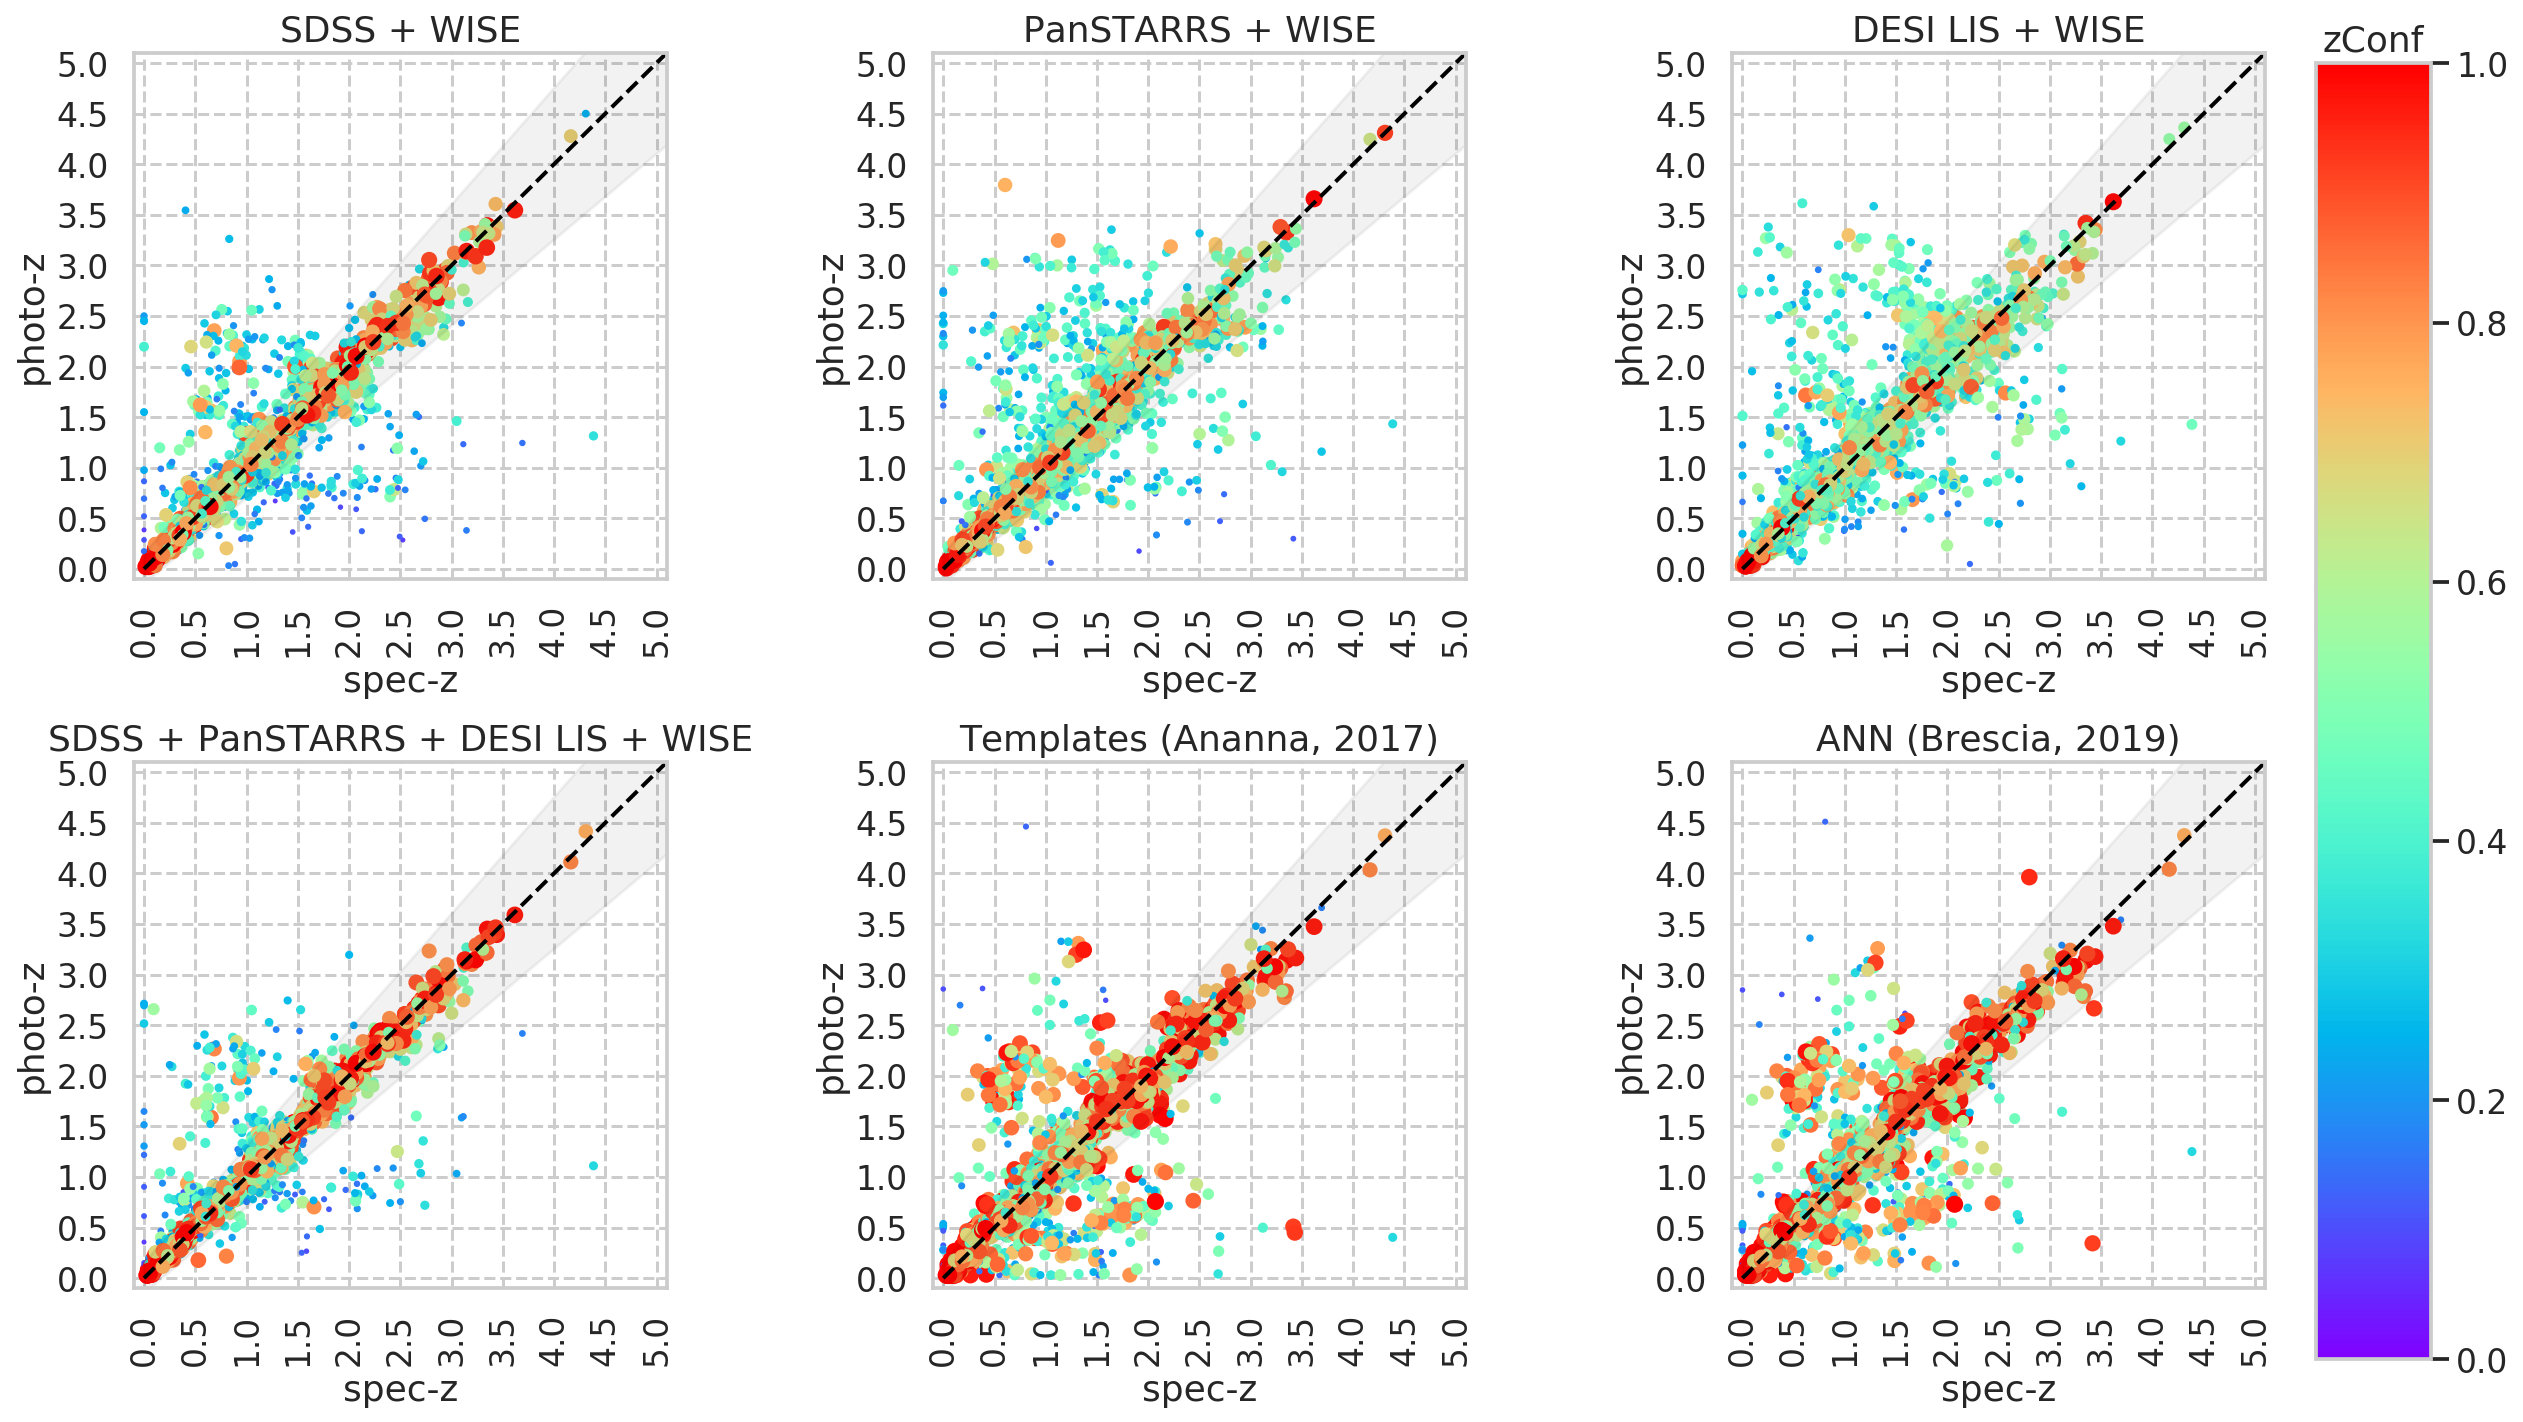
\includegraphics[width=\linewidth]{images/scatterplots-s82x-a17-all30sec.png}
    \caption{Scatterplots on Stripe82X-A17}
    \label{fig:my_label}
\end{figure*}

\begin{figure}
    \centering
    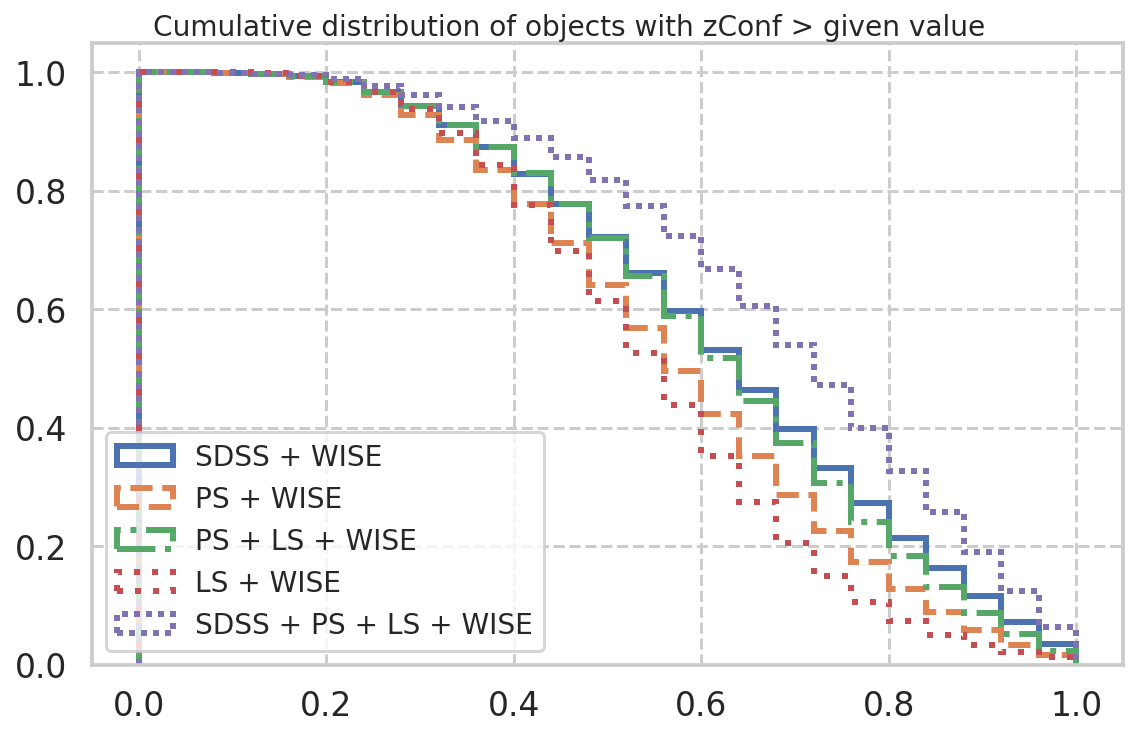
\includegraphics[width=\linewidth]{images/zconfs2-dr16qso.png}
    \caption{zConf cumulative distribution for DR16 qso test}
    \label{fig:zconfs2-dr16qso}
\end{figure}

\subsubsection{Quality of confidence intervals}

То же самое, но по метрикам Колмогорова-Смирнова, квантильный график для доверительных интервалов, сравнение с Ananna и Brescia (они приводят доверительные инттервалы?)

\begin{figure*}
    \centering
    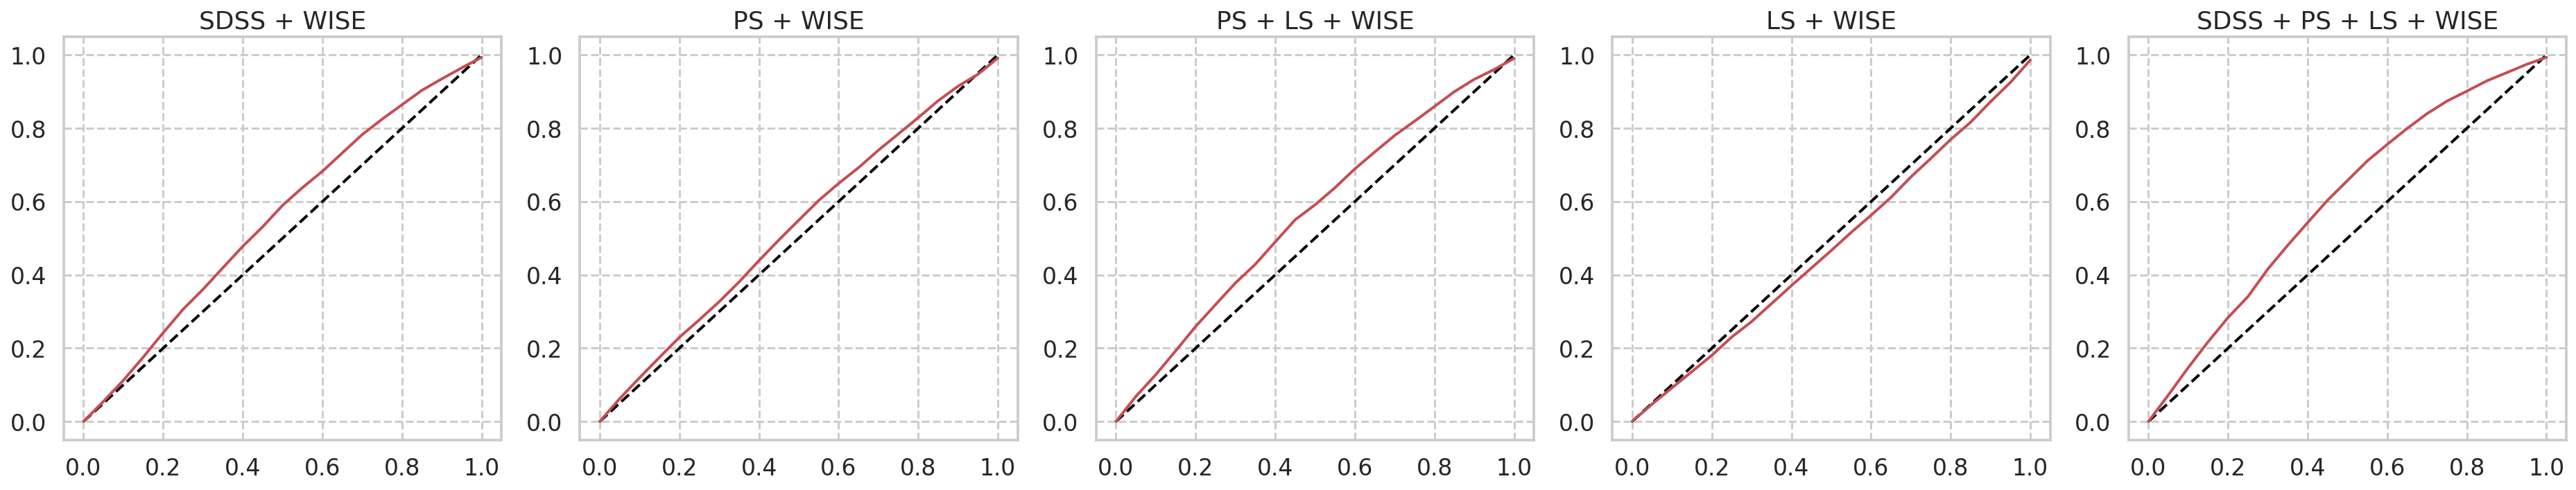
\includegraphics[width=\linewidth]{images/calibration-ci.png}
    \caption{QQ-plot for confidence intervals on Stripe82X test.}
    \label{fig:qqci}
\end{figure*}


\begin{figure*}
    \centering
    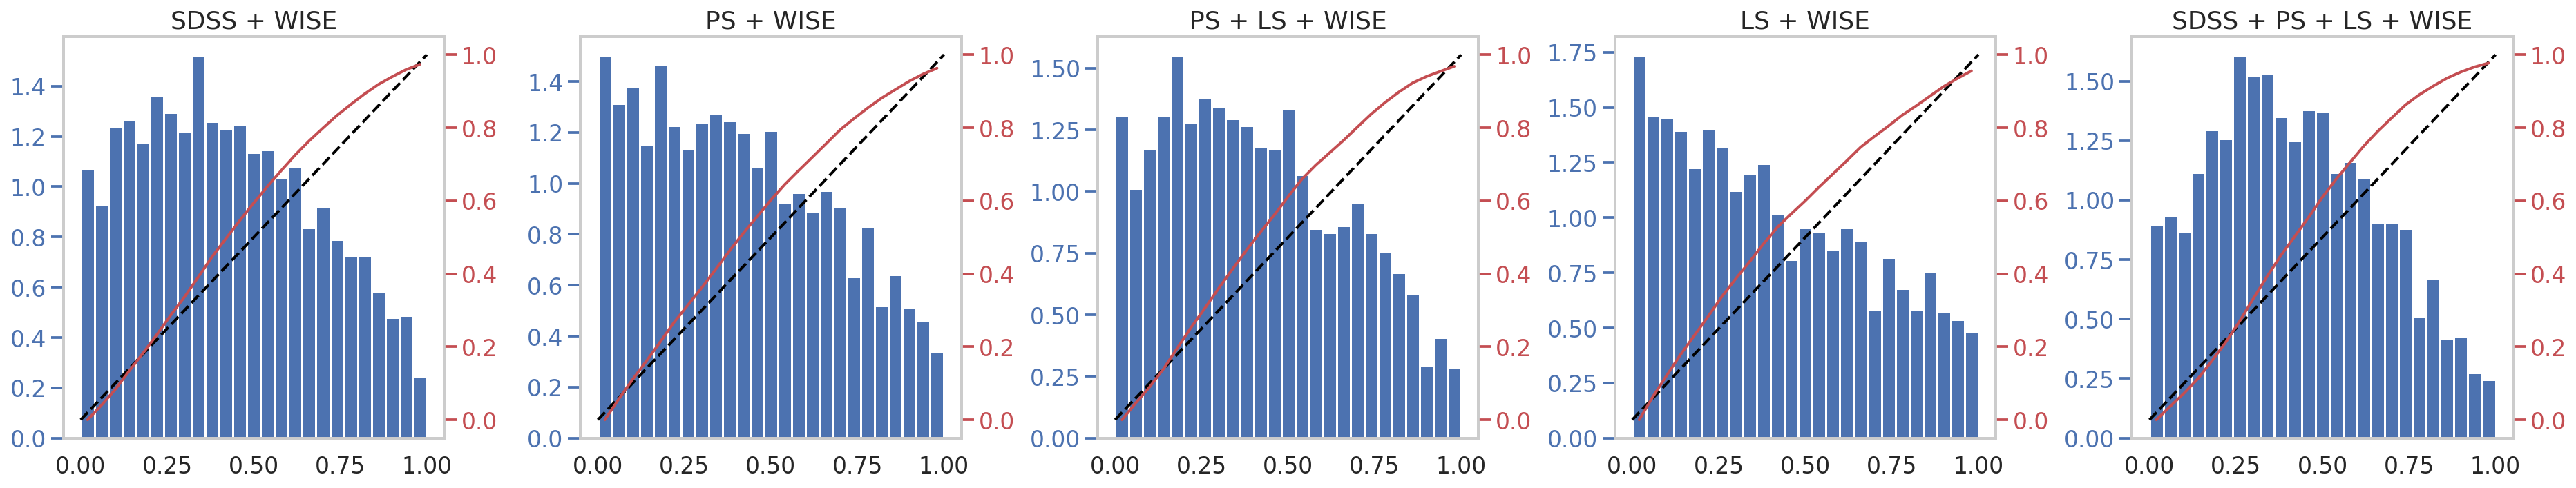
\includegraphics[width=\linewidth]{images/calibration-pit.png}
    \caption{PIT-histogram and QQ-plot for full probabilistic predictions on Stripe82X test.}
    \label{fig:qqpit}
\end{figure*}

Доверительные интервалы немного самоуверенные. Чем точнее модель, тем хуже калибровка.